\documentclass[a4paper]{article}
\usepackage{booktabs,dcolumn,multicol,parskip,graphicx,color,soul,datetime,tocloft,float}
\usepackage[pdfstartview=FitPage, colorlinks=true, linkcolor=black, citecolor=blue, urlcolor=blue, linktoc=all]{hyperref}
\newcolumntype{d}[1]{D{,}{.}{#1}}
\parskip=\baselineskip
\parindent=0pt
\setlength\belowcaptionskip{.075cm}
\begin{document}

{\centering
\hbox{}
\vspace{6cm}
{\Large\scshape Bibliometric Data Exploration\par}
\vspace{1cm}
{\Huge\bfseries Analysis Report\par}
\vspace{1.5cm}
\setlength{\parskip}{0pt}
{\Large\itshape Article database \par jdbc:mysql://localhost:3306/bibxdb \par}
\vspace{6cm}
\setlength{\parskip}{4pt}
{\Large{\itshape Generated by} BibX\footnote{\href{http://github.com/mkkln/bibx}{http://github.com/mkkln/bibx}} {\itshape on:}\par}
% datetime settings:
\renewcommand{\dateseparator}{.}
\settimeformat{hhmmsstime}
\ddmmyyyydate
{\large\today{ at }\currenttime\par}
} % centering
\thispagestyle{empty}
\enlargethispage{2.5 \baselineskip}
\clearpage

\hbox{}
\thispagestyle{empty}
\clearpage

\pagenumbering{roman}
\setlength\cftaftertoctitleskip{5ex}
\tableofcontents
\clearpage

\pagenumbering{arabic}
\section{Summary statistics}

Database: jdbc:mysql://localhost:3306/bibxdb?useSSL=false

Article count: 327\\
\hspace*{0.5cm} Total number of article pages: 5791\\
\hspace*{0.5cm} Average number of pages per article: 17.71

Unique author count: 705\\
\hspace*{0.5cm} Article-author relation count: 825\\
\hspace*{0.5cm} Average number of authors per article: 2.52\\
Unique author address count: 693\\
\hspace*{0.5cm} Article-address relation count: 717\\
\hspace*{0.5cm} Average number of addresses per article: 2.19

Unique source count: 150

Unique source WoS category count: 34\\
\hspace*{0.5cm} Source-source\_category relation count: 264\\
\hspace*{0.5cm} Average number of source WoS categories per source: 1.76\\
\hspace*{0.5cm} Source-source\_category relation count, weighted by source count: 610\\
Unique source research area count: 22\\
\hspace*{0.5cm} Source-source\_area relation count: 219\\
\hspace*{0.5cm} Average number of source research areas per source: 1.46\\
\hspace*{0.5cm} Source-source\_area relation count, weighted by source count: 495

Unique author keyword count: 750\\
\hspace*{0.5cm} Article-author\_keyword relation count: 1258\\
\hspace*{0.5cm} Average number of author keywords per article: 3.85\\
Unique keyword plus count: 789\\
\hspace*{0.5cm} Article-keyword\_plus relation count: 2873\\
\hspace*{0.5cm} Average number of keyword plus per article: 8.79

Unique cited reference count: 12780\\
\hspace*{0.5cm} Article-cited\_reference relation count: 22367\\
\hspace*{0.5cm} Average number of cited references per article: 68.40

Citations to the articles: 20315\\
\hspace*{0.5cm} Average number of citations per article: 62.13

\clearpage

\section{Articles}

\begin{table}[H]
\centering
\caption{Number of articles per year (all years included)}
\begin{tabular}{*{2}{r}d{2}}
\toprule
\multicolumn{1}{r}{Year}&\multicolumn{1}{r}{Count}&\multicolumn{1}{r}{\%} \\
\midrule
2016 & 13 & 3,98\\
2015 & 40 & 12,23\\
2014 & 50 & 15,29\\
2013 & 44 & 13,46\\
2012 & 30 & 9,17\\
2011 & 30 & 9,17\\
2010 & 23 & 7,03\\
2009 & 20 & 6,12\\
2008 & 21 & 6,42\\
2007 & 11 & 3,36\\
2006 & 10 & 3,06\\
2005 & 13 & 3,98\\
2004 & 4 & 1,22\\
2003 & 5 & 1,53\\
2002 & 3 & 0,92\\
2001 & 4 & 1,22\\
2000 & 1 & 0,31\\
1999 & 1 & 0,31\\
1998 & 2 & 0,61\\
1996 & 1 & 0,31\\
1990 & 1 & 0,31\\
Total & 327 & 100,00\\
\bottomrule
\end{tabular}
\end{table}

\hbox{}

\begin{figure}[hb]
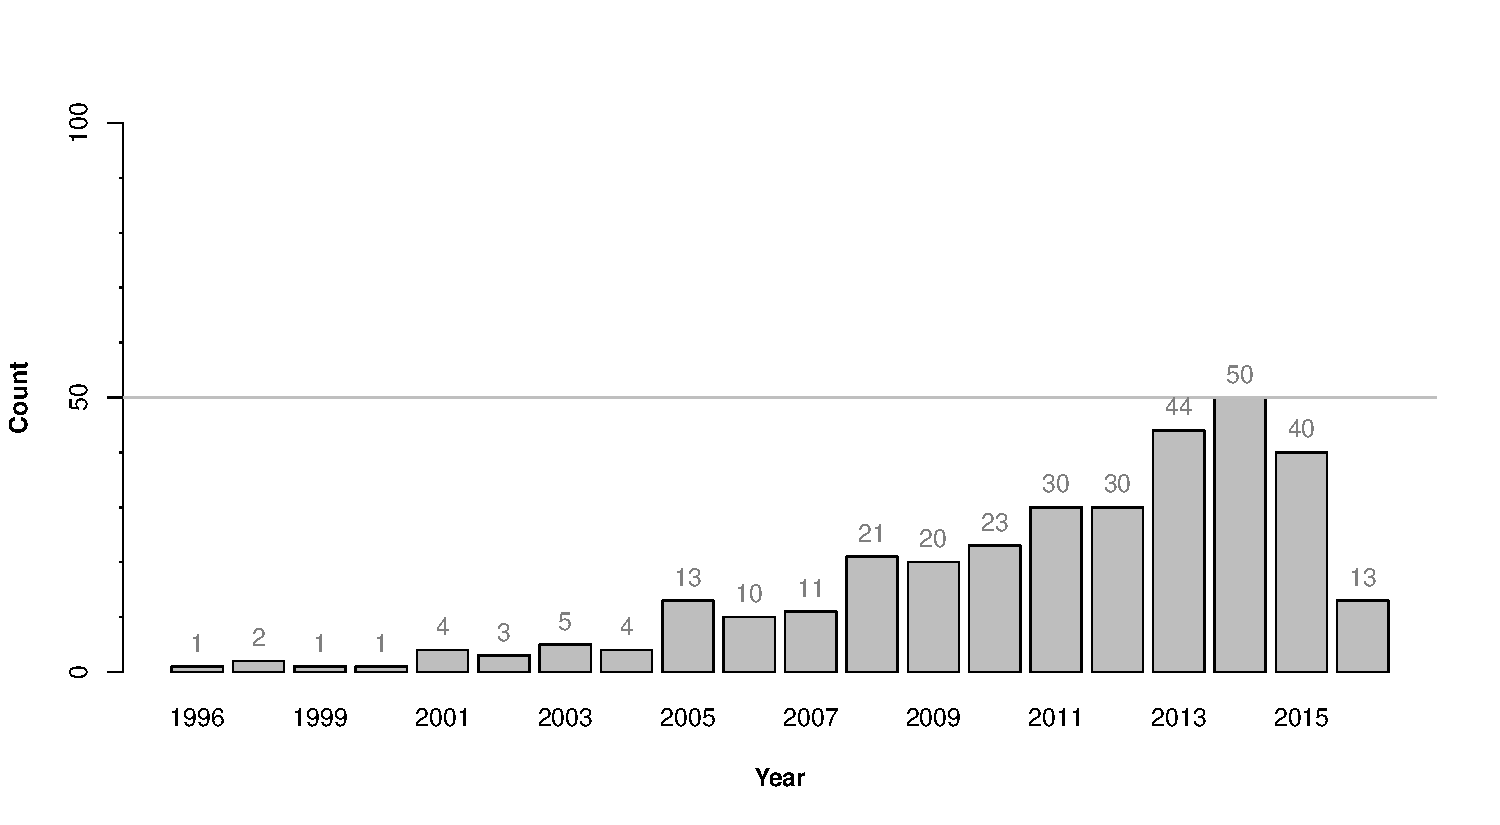
\includegraphics[width=\textwidth]{report_files/bibx_report_bar-years.pdf}
\caption{Articles per year (20 most recent years)}
\end{figure}

\clearpage

\begin{table}[htbp]
\centering
\caption{Number of articles per type}
\begin{tabular}{*{2}{r}d{2}}
\toprule
\multicolumn{1}{r}{Type}&\multicolumn{1}{r}{Count}&\multicolumn{1}{r}{\%} \\
\midrule
Article & 295 & 90,21\\
Review & 18 & 5,50\\
Article; Proceedings Paper & 13 & 3,98\\
Editorial Material & 1 & 0,31\\
Total & 327 & 100,00\\
\bottomrule
\end{tabular}
\end{table}

\hbox{}

\begin{figure}[hb]
\makebox[\textwidth][c]{
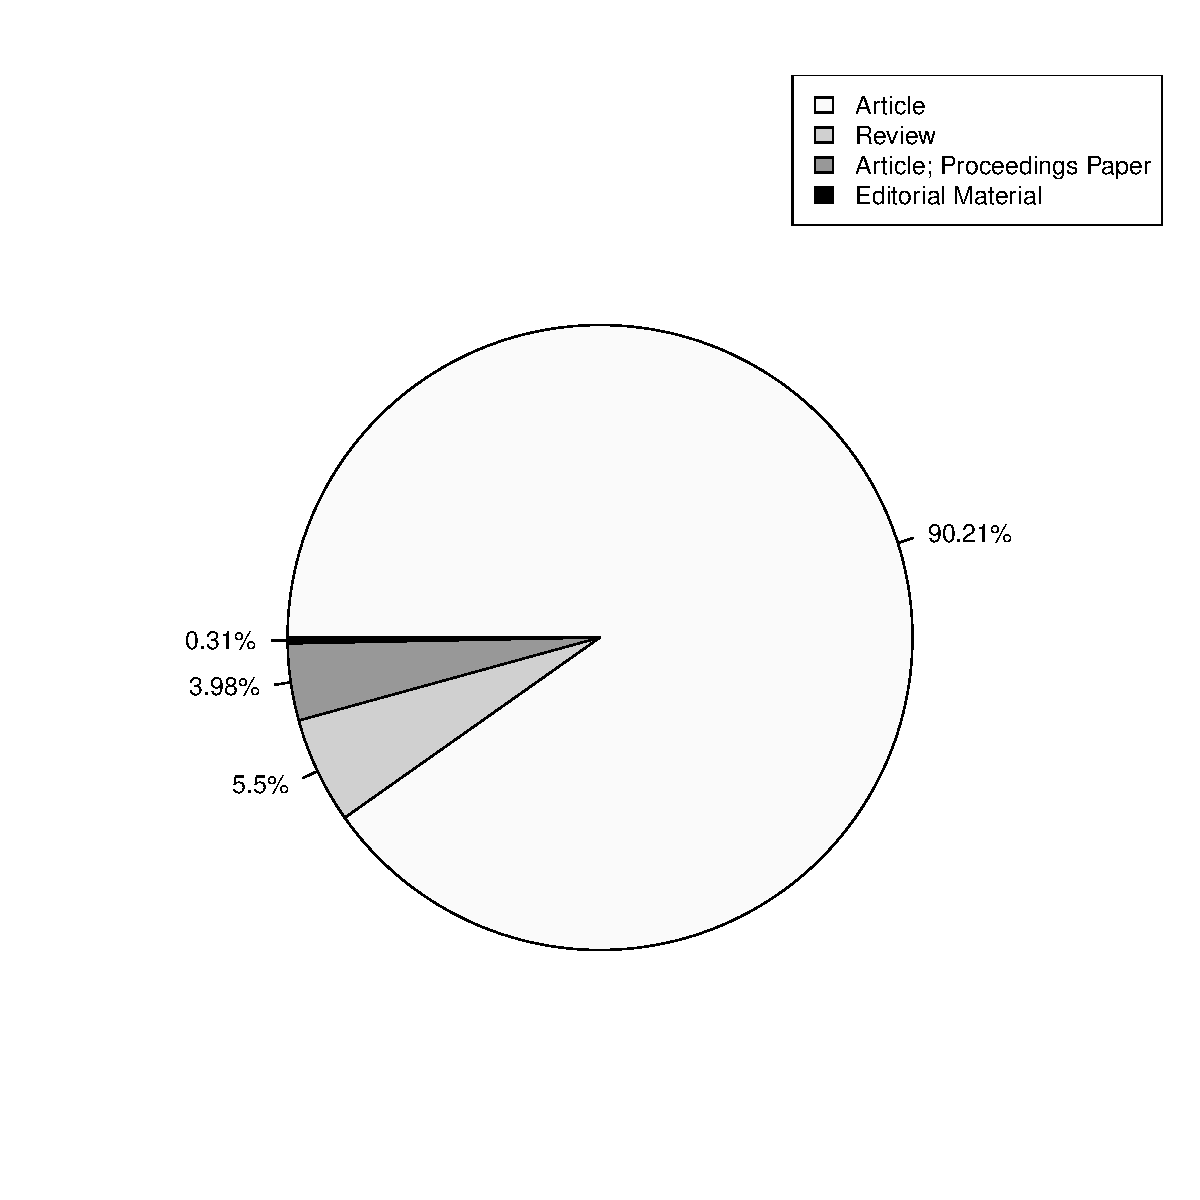
\includegraphics[width=0.75\textwidth]{report_files/bibx_report_pie-type.pdf}
}
\caption{Articles per type}
\end{figure}

\clearpage

\begin{table}[htbp]
\centering
\caption{10 most cited articles}
\footnotesize\rotatebox{90}{\begin{tabular}{p{4cm}rp{9cm}p{3cm}r}
\toprule
\multicolumn{1}{l}{Author(s)} & \multicolumn{1}{r}{Year} & \multicolumn{1}{l}{Title} & \multicolumn{1}{l}{Source} & \multicolumn{1}{r}{Cited} \\
\midrule
\rule{0pt}{3ex}COHEN, LEVINTHAL & 1990 & ABSORPTIVE-CAPACITY - A NEW PERSPECTIVE ON LEARNING AND INNOVATION & Administrative science quarterly & 7703 \\
\rule{0pt}{3ex}Zahra, George & 2002 & Absorptive capacity: A review, reconceptualization, and extension & Academy of management review & 1831 \\
\rule{0pt}{3ex}Lane, Lubatkin & 1998 & Relative absorptive capacity and interorganizational learning & Strategic management journal & 1300 \\
\rule{0pt}{3ex}Tsai & 2001 & Knowledge transfer in intraorganizational networks: Effects of network position and absorptive capacity on business unit innovation and performance & Academy of management journal & 933 \\
\rule{0pt}{3ex}Lane, Salk, Lyles & 2001 & Absorptive capacity, learning, and performance in international joint ventures & Strategic management journal & 540 \\
\rule{0pt}{3ex}Lane, Koka, Pathak & 2006 & The reification of absorptive capacity: A critical review and rejuvenation of the construct & Academy of management review & 455 \\
\rule{0pt}{3ex}Jansen, Van den Bosch, Volberda & 2005 & Managing potential and realized absorptive capacity: How do organizational antecedent's matter? & Academy of management journal & 371 \\
\rule{0pt}{3ex}Cockburn, Henderson & 1998 & Absorptive capacity, coauthoring behavior, and the organization of research in drug discovery & Journal of industrial economics & 354 \\
\rule{0pt}{3ex}Van den Bosch, Volberda, de Boer & 1999 & Coevolution of firm absorptive capacity and knowledge environment: Organizational forms and combinative capabilities & Organization science & 331 \\
\rule{0pt}{3ex}Minbaeva, Pedersen, Bjorkman, Fey, Park & 2003 & MNC knowledge transfer, subsidiary absorptive capacity, and HRM & Journal of international business studies & 304 \\
... & & & & ... \\
Total & & & & 20315 \\
\bottomrule
\end{tabular}
} % rotatebox
\end{table}

\clearpage

\section{Authors}

\begin{table}[htbp]
\centering
\caption{Number of articles per author count}
\begin{tabular}{lrd{2}}
\toprule
\multicolumn{1}{l}{Authors}&\multicolumn{1}{r}{Count}&\multicolumn{1}{r}{\%} \\
\midrule
1 & 50 & 15,29\\
2 & 116 & 35,47\\
3 & 108 & 33,03\\
4 & 46 & 14,07\\
5 & 7 & 2,14\\
Total & 327 & 100,00\\
\bottomrule
\end{tabular}
\end{table}

\begin{figure}[H]
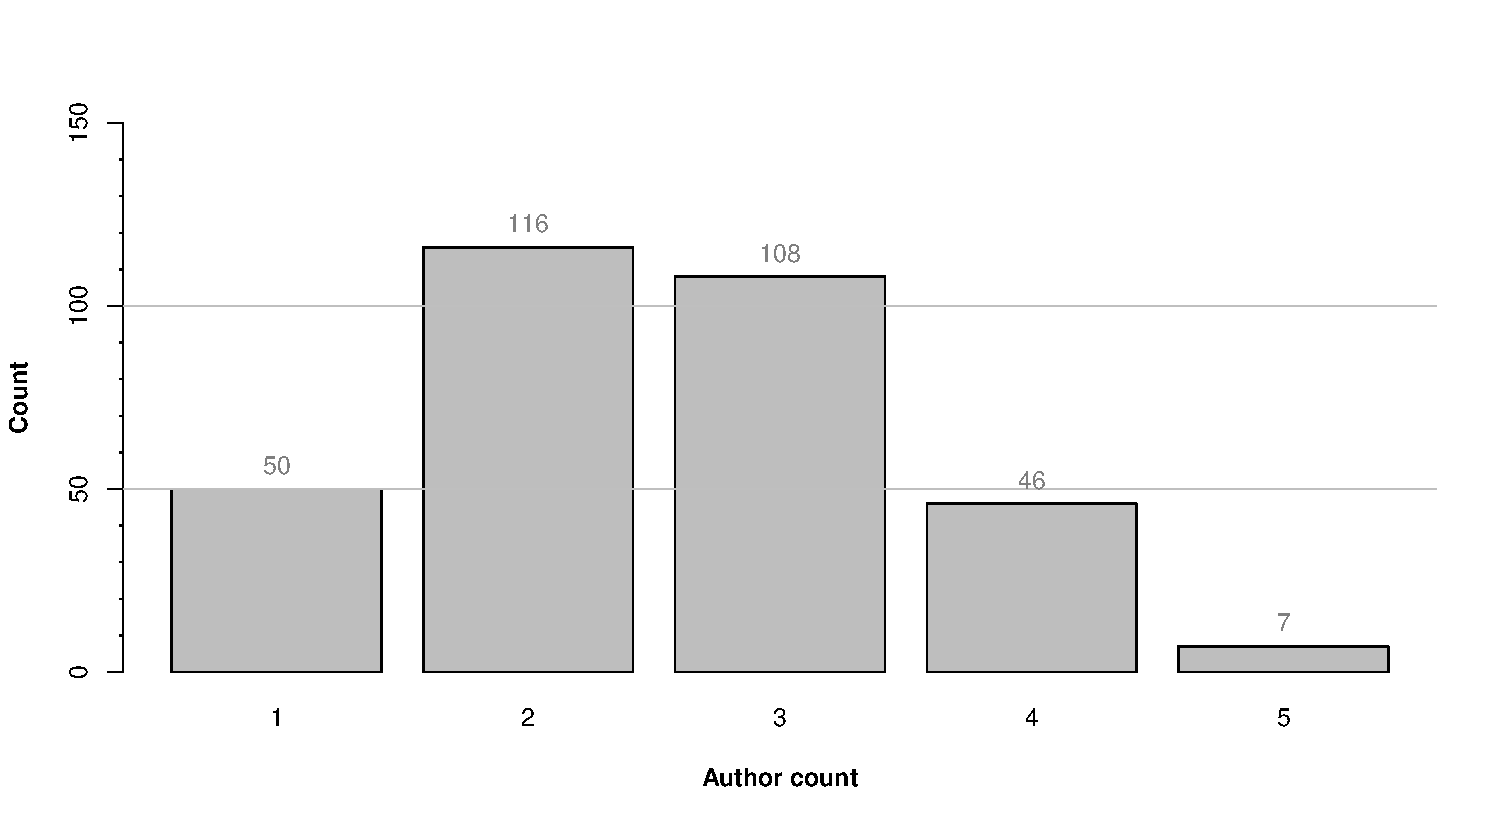
\includegraphics[width=\textwidth]{report_files/bibx_report_bar-author-count.pdf}
\caption{Articles per author count}
\end{figure}

\clearpage

\begin{table}[htbp]
\centering
\caption{Number of authors with specific author order}
\begin{tabular}{lrd{2}}
\toprule
\multicolumn{1}{l}{Order}&\multicolumn{1}{r}{Count}&\multicolumn{1}{r}{\%} \\
\midrule
1 & 327 & 39,64\\
2 & 277 & 33,58\\
3 & 161 & 19,52\\
4 & 53 & 6,42\\
5 & 7 & 0,85\\
Total & 825 & 100,00\\
\bottomrule
\end{tabular}
\end{table}

\clearpage

\begin{table}[htbp]
\centering
\caption{40 authors with most authorships}
\begin{tabular}{lrd{2}}
\toprule
\multicolumn{1}{l}{Name}&\multicolumn{1}{r}{Count}&\multicolumn{1}{r}{\%} \\
\midrule
Hurmelinna-Laukkanen, P & 5 & 0,61\\
Patel, PC & 5 & 0,61\\
Pedersen, T & 5 & 0,61\\
Zahra, SA & 5 & 0,61\\
Bjorkman, I & 4 & 0,48\\
Chen, YS & 4 & 0,48\\
Garcia-Morales, VJ & 4 & 0,48\\
Volberda, HW & 4 & 0,48\\
Brettel, M & 3 & 0,36\\
Camison, C & 3 & 0,36\\
Chang, CH & 3 & 0,36\\
Fey, CF & 3 & 0,36\\
Flatten, TC & 3 & 0,36\\
Fores, B & 3 & 0,36\\
Gong, YP & 3 & 0,36\\
Knoppen, D & 3 & 0,36\\
Lane, PJ & 3 & 0,36\\
Lichtenthaler, U & 3 & 0,36\\
Lyles, MA & 3 & 0,36\\
McAdam, R & 3 & 0,36\\
Saenz, MJ & 3 & 0,36\\
Van den Bosch, FAJ & 3 & 0,36\\
Akbar, H & 2 & 0,24\\
Al-Dajani, H & 2 & 0,24\\
Anderson, MH & 2 & 0,24\\
Aribi, A & 2 & 0,24\\
Ariza-Montes, JA & 2 & 0,24\\
Azagra-Caro, JM & 2 & 0,24\\
Bolivar-Ramos, MT & 2 & 0,24\\
Cegarra-Navarro, JG & 2 & 0,24\\
Cepeda-Carrion, G & 2 & 0,24\\
Chang, S & 2 & 0,24\\
Clarysse, B & 2 & 0,24\\
Dupouet, O & 2 & 0,24\\
Egbetokun, A & 2 & 0,24\\
Engelen, A & 2 & 0,24\\
Exposito-Langa, M & 2 & 0,24\\
Feeny, S & 2 & 0,24\\
Fernandez-De-Lucio, I & 2 & 0,24\\
Fosfuri, A & 2 & 0,24\\
... & & \\
Total & 825 & 100,00\\
\bottomrule
\multicolumn{3}{l}{\footnotesize Note: Articles can list multiple authors} \\
\end{tabular}
\end{table}

\clearpage

\begin{table}[htbp]
\centering
\caption{10 authors with most first authorships}
\begin{tabular}{lrd{2}}
\toprule
\multicolumn{1}{l}{Name}&\multicolumn{1}{r}{Count}&\multicolumn{1}{r}{\%} \\
\midrule
Chen, YS & 3 & 0,92\\
Hurmelinna-Laukkanen, P & 3 & 0,92\\
Lane, PJ & 3 & 0,92\\
Lichtenthaler, U & 3 & 0,92\\
Zahra, SA & 3 & 0,92\\
Aribi, A & 2 & 0,61\\
Azagra-Caro, JM & 2 & 0,61\\
Camison, C & 2 & 0,61\\
Cepeda-Carrion, G & 2 & 0,61\\
Exposito-Langa, M & 2 & 0,61\\
... & & \\
Total & 327 & 100,00\\
\bottomrule
\end{tabular}
\end{table}

\begin{table}[htbp]
\centering
\caption{10 authors with most second authorships}
\begin{tabular}{lrd{2}}
\toprule
\multicolumn{1}{l}{Name}&\multicolumn{1}{r}{Count}&\multicolumn{1}{r}{\%} \\
\midrule
Pedersen, T & 5 & 1,81\\
Anderson, MH & 2 & 0,72\\
Clarysse, B & 2 & 0,72\\
Dupouet, O & 2 & 0,72\\
Fores, B & 2 & 0,72\\
Garcia-Morales, VJ & 2 & 0,72\\
Gong, YP & 2 & 0,72\\
Hurmelinna-Laukkanen, P & 2 & 0,72\\
Lichtenthaler, E & 2 & 0,72\\
Massini, S & 2 & 0,72\\
... & & \\
Total & 277 & 100,00\\
\bottomrule
\end{tabular}
\end{table}

\begin{table}[H]
\centering
\caption{10 authors with most third authorships}
\begin{tabular}{lrd{2}}
\toprule
\multicolumn{1}{l}{Name}&\multicolumn{1}{r}{Count}&\multicolumn{1}{r}{\%} \\
\midrule
Bjorkman, I & 3 & 1,86\\
Lyles, MA & 3 & 1,86\\
Brettel, M & 2 & 1,24\\
Knockaert, M & 2 & 1,24\\
Knoppen, D & 2 & 1,24\\
Llorens-Montes, FJ & 2 & 1,24\\
Martin-Rojas, R & 2 & 1,24\\
Volberda, HW & 2 & 1,24\\
Akbar, H & 1 & 0,62\\
Antonacopoulou, E & 1 & 0,62\\
... & & \\
Total & 161 & 100,00\\
\bottomrule
\end{tabular}
\end{table}

\clearpage

\begin{figure}[p]
\makebox[\textwidth][c]{
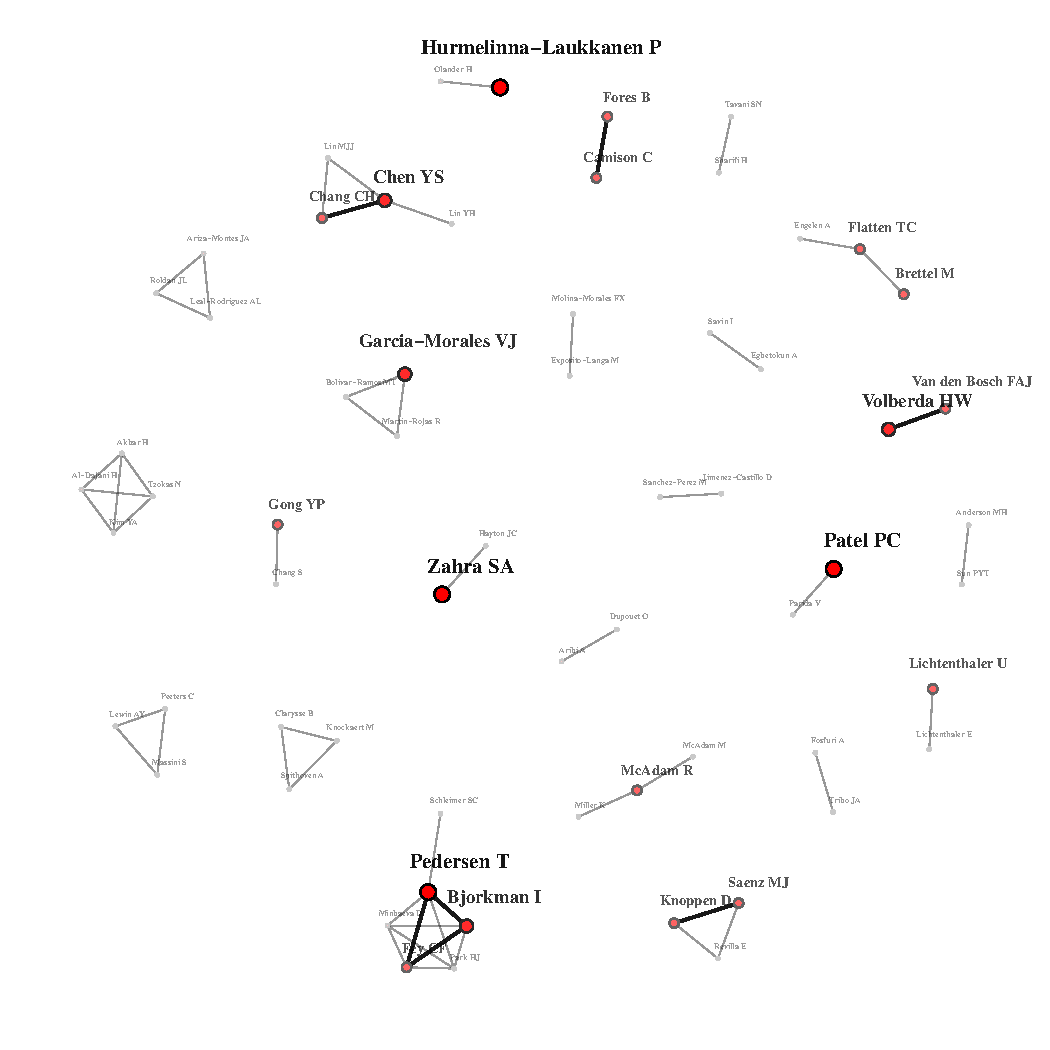
\includegraphics[width=1.5\textwidth]{report_files/bibx_report_net-coauthorships.pdf}
}
\caption{Coauthorship networks (only coauthorships recurring 2 times or more shown)}
\end{figure}

\clearpage

\section{Addresses}

\begin{table}[H]
\centering
\caption{40 most mentioned addresses}
\makebox[\textwidth][c]{
\begin{tabular}{lrd{2}}
\toprule
\multicolumn{1}{l}{Name}&\multicolumn{1}{r}{Count}&\multicolumn{1}{r}{\%} \\
\midrule
NONE & 5 & 0,70\\
{[}Patel, Pankaj C.{]} Ball State Univ, Miller Coll Business, Muncie, IN 47306 USA. & 4 & 0,56\\
{[}Gong, Yaping{]} Hong Kong Univ Sci \& Technol, Hong Kong, Hong Kong, Peoples R China. & 3 & 0,42\\
Natl Cheng Kung Univ, Dept Business Adm, Tainan 70101, Taiwan. & 2 & 0,28\\
Univ Leicester, Dept Econ, Leicester LE1 7RH, Leics, England. & 2 & 0,28\\
Univ So Calif, Marshall Sch Business, Los Angeles, CA 90089 USA. & 2 & 0,28\\
{[}Camison, Cesar; Fores, Beatriz{]} Univ Jaume 1, Dept Business Adm \& Mkt, E-12071 Castellon de La & 2 & 0,28\\
{[}Cepeda-Carrion, Gabriel{]} Univ Seville, Management \& Mkt Dept, Seville 3441018, Spain. & 2 & 0,28\\
{[}Clarysse, Bart; Knockaert, Mirjam{]} Univ Ghent, B-9000 Ghent, Belgium. & 2 & 0,28\\
{[}Clarysse, Bart{]} Univ London Imperial Coll Sci Technol \& Med, Sch Business, London SW7 2AZ, Eng & 2 & 0,28\\
{[}Hurmelinna-Laukkanen, Pia{]} Univ Oulu, Oulu Business Sch, Oulu, Finland. & 2 & 0,28\\
{[}Knockaert, Mirjam{]} Univ Oslo, N-0318 Oslo, Norway. & 2 & 0,28\\
{[}Lichtenthaler, Eckhard{]} Swiss Fed Inst Technol Zurich ETHZ, Zurich, Switzerland. & 2 & 0,28\\
{[}McAdam, Maura{]} Queens Univ Belfast, Sch Management \& Econ, Belfast BT7 1NN, Antrim, North Irel & 2 & 0,28\\
{[}Pedersen, Torben{]} Bocconi Univ, Milan, Italy. & 2 & 0,28\\
{[}Spithoven, Andre{]} Belgian Sci Policy, B-1000 Brussels, Belgium. & 2 & 0,28\\
{[}Spithoven, Andre{]} Vlerick Leuven Gent Management Sch, B-9000 Ghent, Belgium. & 2 & 0,28\\
{[}Sun, Peter Y. T.{]} Univ Waikato, Waikato Management Sch, Hamilton 3240, New Zealand. & 2 & 0,28\\
Arizona State Univ, Coll Business, Tempe, AZ 85287 USA. & 1 & 0,14\\
Arizona State Univ, WP Carey Sch Business, Tempe, AZ 85287 USA. & 1 & 0,14\\
Aston Univ, Aston Business Sch, Birmingham B4 7ET, W Midlands, England. & 1 & 0,14\\
Babson Coll, Arthur M Blank Ctr Enterpreneurship, Babson Pk, MA 02457 USA. & 1 & 0,14\\
Carnegie Mellon Univ, Pittsburgh, PA 15213 USA. & 1 & 0,14\\
Case Western Reserve Univ, Weatherhead Sch Management, Div Entrepreneurship, Cleveland, OH 4410 & 1 & 0,14\\
Chonnam Natl Univ, E Serv Team Free21, Kwangju 500757, South Korea. & 1 & 0,14\\
Colorado Sch Mines, Div Econ \& Business, Golden, CO 80401 USA. & 1 & 0,14\\
Colorado State Univ, Coll Business, Ft Collins, CO 80523 USA. & 1 & 0,14\\
Copenhagen Business Sch, Copenhagen, Denmark. & 1 & 0,14\\
Copenhagen Sch Econ \& Business Adm, Dept Int Econ \& Managment, DK-2000 Copenhagen, Denmark. & 1 & 0,14\\
Cornell Univ, Ithaca, NY 14853 USA. & 1 & 0,14\\
Ctr European Econ Res, D-68161 Mannheim, Germany. & 1 & 0,14\\
Dartmouth Coll, Dept Econ, Hanover, NH 03755 USA. & 1 & 0,14\\
Dartmouth Coll, Tuck Sch Business, Hanover, NH USA. & 1 & 0,14\\
Depaul Univ, Dept Management, Chicago, IL 60604 USA. & 1 & 0,14\\
Dept Strategy \& Management, Grp ESSEC, Cergy Pontoise, France. & 1 & 0,14\\
Duke Univ, Fuqua Sch Business, Durham, NC 27708 USA. & 1 & 0,14\\
Ecole Management Lyon, Lyon, France. & 1 & 0,14\\
Ecole Polytech Fed Lausanne, Coll Management Technol, MTEI CEMI, EPFL, CH-1015 Lausanne, Switze & 1 & 0,14\\
Eindhoven Univ Technol, ECIS, NL-5612 AZ Eindhoven, Netherlands. & 1 & 0,14\\
Erasmus Univ, Dept Mkt Management, Rotterdam, Netherlands. & 1 & 0,14\\
... & & \\
Total & 717 & 100,00\\
\bottomrule
\multicolumn{3}{l}{\footnotesize Note: Articles can list multiple addresses} \\
\end{tabular}
}
\end{table}

\clearpage

\begin{table}[htbp]
\centering
\caption{40 most mentioned countries in the addresses}
\makebox[\textwidth][c]{
\begin{tabular}{lrd{2}}
\toprule
\multicolumn{1}{l}{Name}&\multicolumn{1}{r}{Count}&\multicolumn{1}{r}{\%} \\
\midrule
USA & 143 & 19,94\\
Spain & 82 & 11,44\\
England & 70 & 9,76\\
Taiwan & 48 & 6,69\\
Peoples R China & 35 & 4,88\\
Netherlands & 33 & 4,60\\
Germany & 32 & 4,46\\
Italy & 26 & 3,63\\
Finland & 25 & 3,49\\
France & 25 & 3,49\\
Australia & 24 & 3,35\\
Belgium & 19 & 2,65\\
South Korea & 19 & 2,65\\
Canada & 18 & 2,51\\
Denmark & 11 & 1,53\\
Norway & 11 & 1,53\\
Switzerland & 11 & 1,53\\
North Ireland & 8 & 1,12\\
Sweden & 8 & 1,12\\
Austria & 6 & 0,84\\
NONE & 5 & 0,70\\
Portugal & 5 & 0,70\\
Russia & 5 & 0,70\\
Scotland & 5 & 0,70\\
Israel & 4 & 0,56\\
Japan & 4 & 0,56\\
Poland & 4 & 0,56\\
Slovenia & 4 & 0,56\\
Colombia & 3 & 0,42\\
New Zealand & 3 & 0,42\\
Thailand & 3 & 0,42\\
Ecuador & 2 & 0,28\\
Greece & 2 & 0,28\\
Ireland & 2 & 0,28\\
Serbia & 2 & 0,28\\
Singapore & 2 & 0,28\\
Iran & 1 & 0,14\\
Kazakhstan & 1 & 0,14\\
Nigeria & 1 & 0,14\\
Saudi Arabia & 1 & 0,14\\
... & & \\
Total & 717 & 100,00\\
\bottomrule
\multicolumn{3}{l}{\footnotesize Note: Articles can list multiple addresses} \\
\end{tabular}
}
\end{table}

\clearpage

\begin{table}[htbp]
\centering
\caption{40 most mentioned countries in the addresses, U.S. states separated}
\makebox[\textwidth][c]{
\begin{tabular}{lrd{2}}
\toprule
\multicolumn{1}{l}{Name}&\multicolumn{1}{r}{Count}&\multicolumn{1}{r}{\%} \\
\midrule
Spain & 82 & 11,44\\
England & 70 & 9,76\\
Taiwan & 48 & 6,69\\
Peoples R China & 35 & 4,88\\
Netherlands & 33 & 4,60\\
Germany & 32 & 4,46\\
Italy & 26 & 3,63\\
Finland & 25 & 3,49\\
France & 25 & 3,49\\
Australia & 24 & 3,35\\
Belgium & 19 & 2,65\\
South Korea & 19 & 2,65\\
Canada & 18 & 2,51\\
Denmark & 11 & 1,53\\
IN USA & 11 & 1,53\\
Norway & 11 & 1,53\\
Switzerland & 11 & 1,53\\
NY USA & 9 & 1,26\\
TX USA & 9 & 1,26\\
MA USA & 8 & 1,12\\
North Ireland & 8 & 1,12\\
OH USA & 8 & 1,12\\
PA USA & 8 & 1,12\\
Sweden & 8 & 1,12\\
GA USA & 7 & 0,98\\
Austria & 6 & 0,84\\
CA USA & 6 & 0,84\\
MN USA & 6 & 0,84\\
NC USA & 6 & 0,84\\
AZ USA & 5 & 0,70\\
CO USA & 5 & 0,70\\
IL USA & 5 & 0,70\\
MI USA & 5 & 0,70\\
NONE & 5 & 0,70\\
Portugal & 5 & 0,70\\
Russia & 5 & 0,70\\
Scotland & 5 & 0,70\\
VA USA & 5 & 0,70\\
Israel & 4 & 0,56\\
Japan & 4 & 0,56\\
... & & \\
Total & 717 & 100,00\\
\bottomrule
\multicolumn{3}{l}{\footnotesize Note: Articles can list multiple addresses} \\
\end{tabular}
}
\end{table}

\clearpage

\begin{table}[htbp]
\centering
\caption{40 most mentioned countries in the addresses, U.S. states and zip codes separated}
\makebox[\textwidth][c]{
\begin{tabular}{lrd{2}}
\toprule
\multicolumn{1}{l}{Name}&\multicolumn{1}{r}{Count}&\multicolumn{1}{r}{\%} \\
\midrule
Spain & 82 & 11,44\\
England & 70 & 9,76\\
Taiwan & 48 & 6,69\\
Peoples R China & 35 & 4,88\\
Netherlands & 33 & 4,60\\
Germany & 32 & 4,46\\
Italy & 26 & 3,63\\
Finland & 25 & 3,49\\
France & 25 & 3,49\\
Australia & 24 & 3,35\\
Belgium & 19 & 2,65\\
South Korea & 19 & 2,65\\
Canada & 18 & 2,51\\
Denmark & 11 & 1,53\\
Norway & 11 & 1,53\\
Switzerland & 11 & 1,53\\
North Ireland & 8 & 1,12\\
Sweden & 8 & 1,12\\
Austria & 6 & 0,84\\
MN 55455 USA & 6 & 0,84\\
IN 47306 USA & 5 & 0,70\\
NONE & 5 & 0,70\\
Portugal & 5 & 0,70\\
Russia & 5 & 0,70\\
Scotland & 5 & 0,70\\
Israel & 4 & 0,56\\
Japan & 4 & 0,56\\
Poland & 4 & 0,56\\
Slovenia & 4 & 0,56\\
Colombia & 3 & 0,42\\
GA 30303 USA & 3 & 0,42\\
MA 02138 USA & 3 & 0,42\\
New Zealand & 3 & 0,42\\
NJ 08855 USA & 3 & 0,42\\
NY 14853 USA & 3 & 0,42\\
OH 43606 USA & 3 & 0,42\\
Thailand & 3 & 0,42\\
AK USA & 2 & 0,28\\
AZ 85287 USA & 2 & 0,28\\
AZ USA & 2 & 0,28\\
... & & \\
Total & 717 & 100,00\\
\bottomrule
\multicolumn{3}{l}{\footnotesize Note: Articles can list multiple addresses} \\
\end{tabular}
}
\end{table}

\clearpage

\begin{figure}[p]
\makebox[\textwidth][c]{
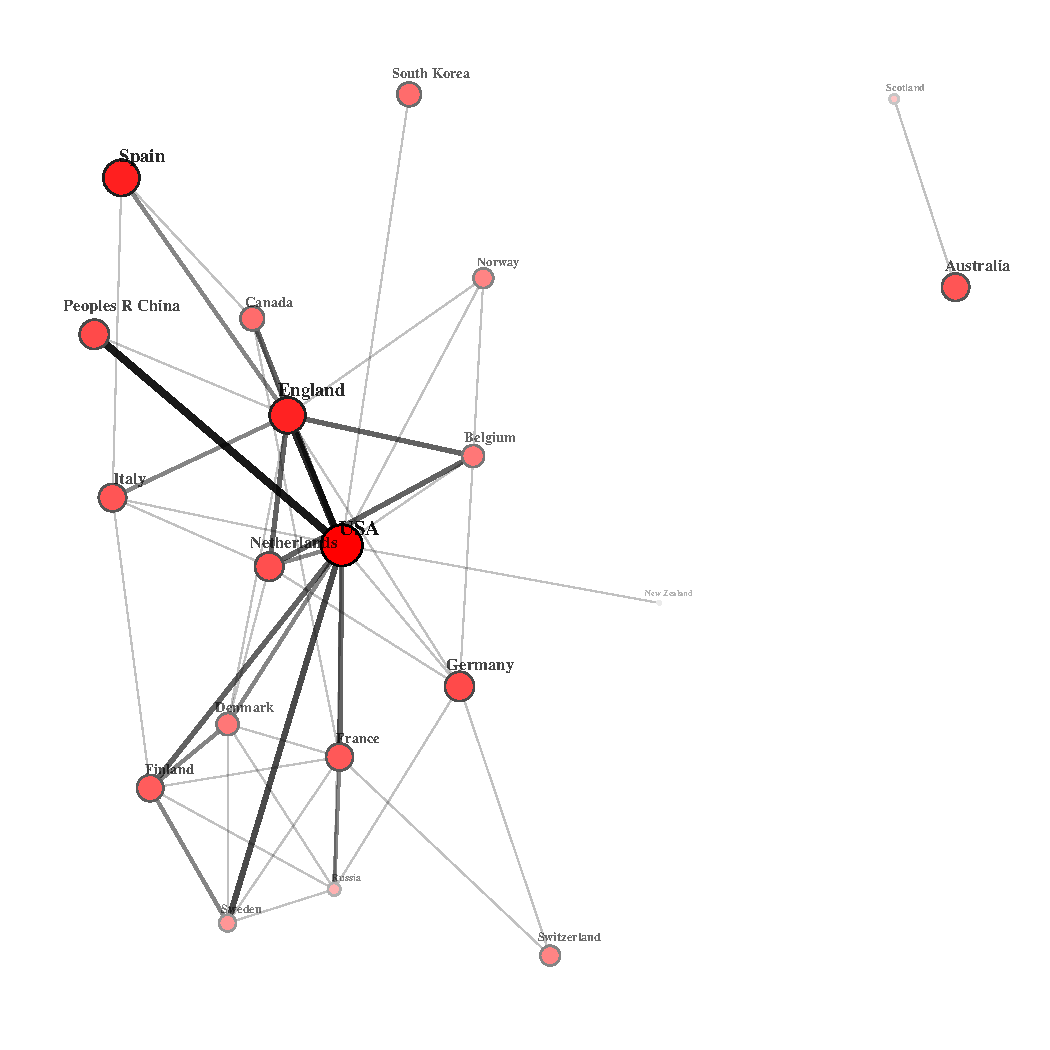
\includegraphics[width=1.5\textwidth]{report_files/bibx_report_net-country-ties.pdf}
}
\caption{Country ties (only ties recurring 2 times or more shown)}
\end{figure}

\clearpage

\begin{figure}[p]
\makebox[\textwidth][c]{
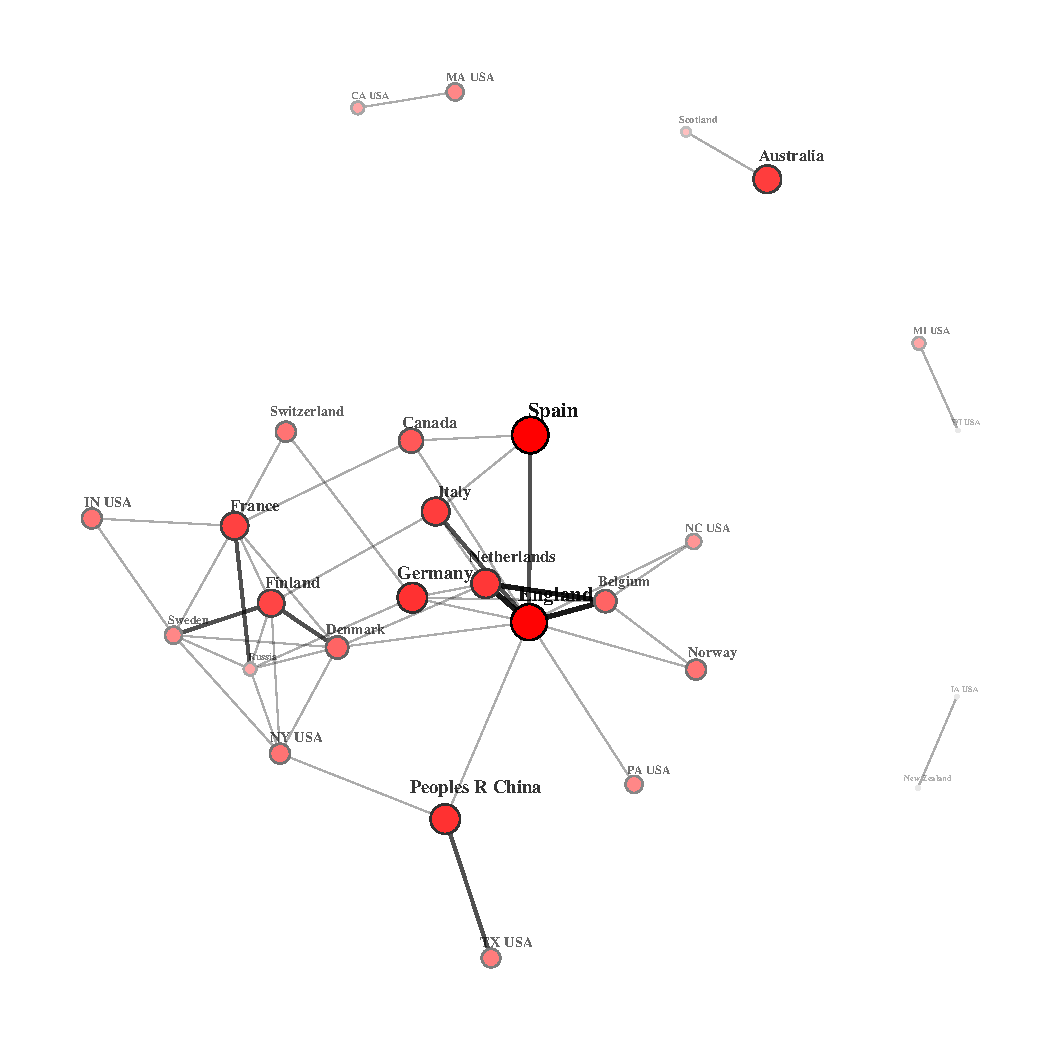
\includegraphics[width=1.5\textwidth]{report_files/bibx_report_net-country-ties-states.pdf}
}
\caption{Country ties, U.S. states separated (only ties recurring 2 times or more shown)}
\end{figure}

\clearpage

\begin{figure}[p]
\makebox[\textwidth][c]{
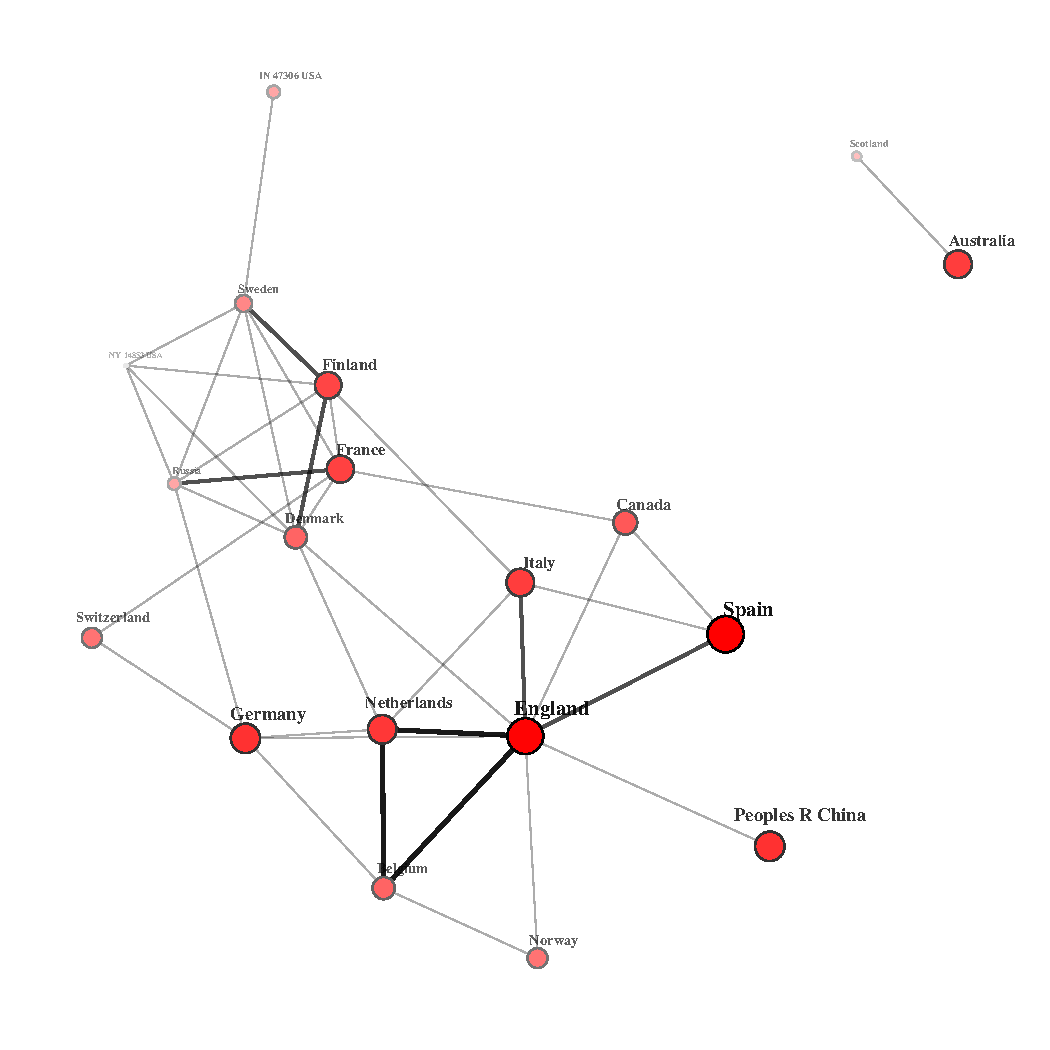
\includegraphics[width=1.5\textwidth]{report_files/bibx_report_net-country-ties-states-zips.pdf}
}
\caption{Country ties, U.S. states and zip codes separated (only ties recurring 2 times or more shown)}
\end{figure}

\clearpage

\begin{table}[htbp]
\centering
\caption{40 most mentioned institutions in the addresses}
\makebox[\textwidth][c]{
\begin{tabular}{lrd{2}}
\toprule
\multicolumn{1}{l}{Name}&\multicolumn{1}{r}{Count}&\multicolumn{1}{r}{\%} \\
\midrule
Erasmus Univ & 8 & 1,12\\
Natl Cheng Kung Univ & 8 & 1,12\\
Univ Nottingham & 8 & 1,12\\
Copenhagen Business Sch & 6 & 0,84\\
Univ Granada & 6 & 0,84\\
Univ Minnesota & 6 & 0,84\\
Univ Politecn Valencia & 6 & 0,84\\
Ball State Univ & 5 & 0,70\\
Indiana Univ & 5 & 0,70\\
Lappeenranta Univ Technol & 5 & 0,70\\
Natl Cent Univ & 5 & 0,70\\
NONE & 5 & 0,70\\
Stockholm Sch Econ & 5 & 0,70\\
Univ Jaume 1 & 5 & 0,70\\
Univ Oulu & 5 & 0,70\\
Univ Ulster & 5 & 0,70\\
Univ Zaragoza & 5 & 0,70\\
Georgia State Univ & 4 & 0,56\\
Tamkang Univ & 4 & 0,56\\
Tampere Univ Technol & 4 & 0,56\\
Univ E Anglia & 4 & 0,56\\
Univ Liverpool & 4 & 0,56\\
Univ Loyola Andalucia & 4 & 0,56\\
Univ Seville & 4 & 0,56\\
Univ Sussex & 4 & 0,56\\
Univ Toledo & 4 & 0,56\\
Aalto Univ & 3 & 0,42\\
Aix Marseille Univ & 3 & 0,42\\
Arizona State Univ & 3 & 0,42\\
Bocconi Univ & 3 & 0,42\\
Chinese Univ Hong Kong & 3 & 0,42\\
City Univ Hong Kong & 3 & 0,42\\
Cornell Univ & 3 & 0,42\\
Duke Univ & 3 & 0,42\\
Griffith Univ & 3 & 0,42\\
Hong Kong Univ Sci \& Technol & 3 & 0,42\\
INSEAD & 3 & 0,42\\
Iowa State Univ & 3 & 0,42\\
Maastricht Univ & 3 & 0,42\\
Natl Taipei Univ & 3 & 0,42\\
... & & \\
Total & 717 & 100,00\\
\bottomrule
\multicolumn{3}{l}{\footnotesize Note: Articles can list multiple addresses} \\
\end{tabular}
}
\end{table}

\clearpage

\begin{figure}[p]
\makebox[\textwidth][c]{
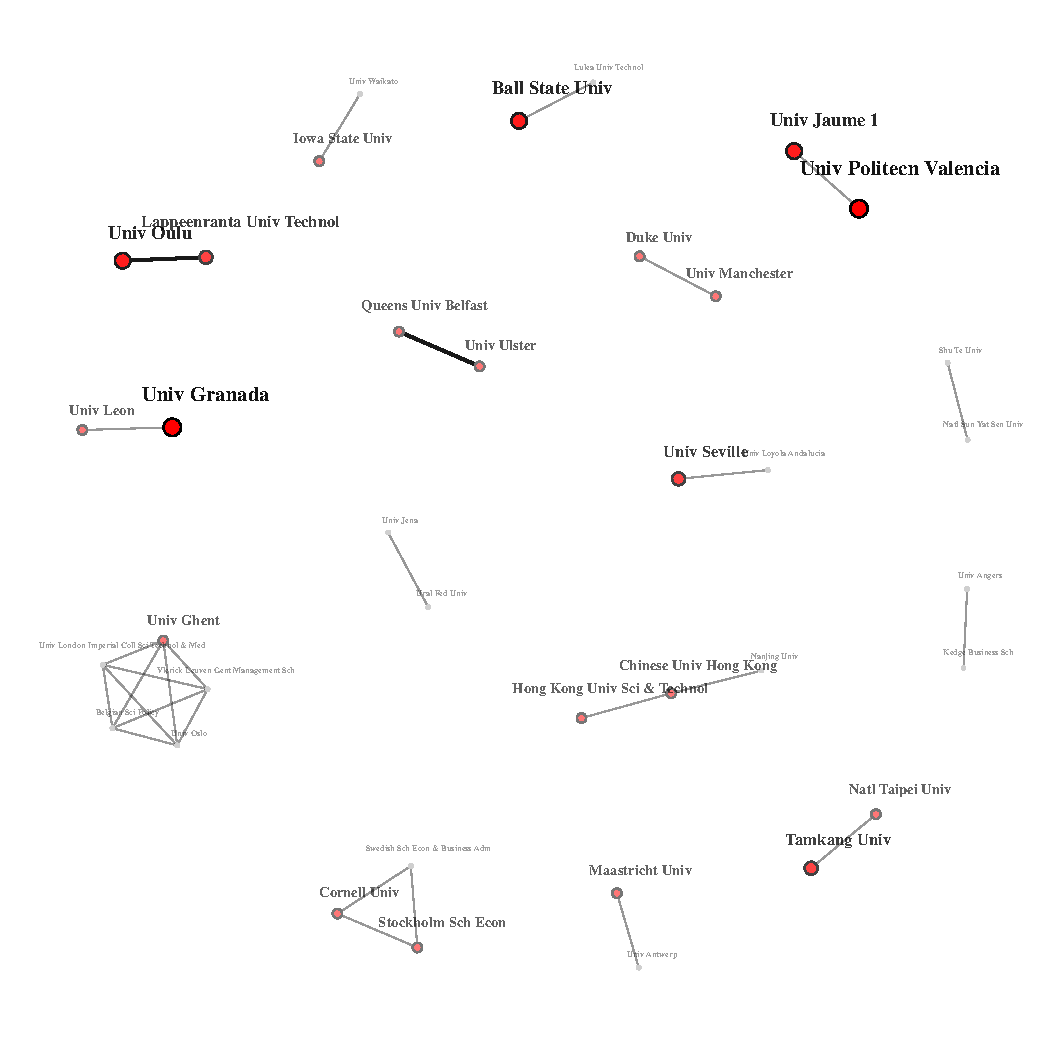
\includegraphics[width=1.5\textwidth]{report_files/bibx_report_net-institutional-ties.pdf}
}
\caption{Institutional ties (only ties recurring 2 times or more shown)}
\end{figure}

\clearpage

\section{Sources}

\begin{table}[H]
\centering
\caption{40 sources with most articles}
\makebox[\textwidth][c]{
\begin{tabular}{lrd{2}}
\toprule
\multicolumn{1}{l}{Name}&\multicolumn{1}{r}{Count}&\multicolumn{1}{r}{\%} \\
\midrule
Research policy & 15 & 4,59\\
Strategic management journal & 11 & 3,36\\
Technovation & 11 & 3,36\\
R \& d management & 10 & 3,06\\
Journal of business research & 8 & 2,45\\
European management journal & 7 & 2,14\\
Technology analysis \& strategic management & 7 & 2,14\\
Industrial marketing management & 6 & 1,83\\
Journal of international business studies & 6 & 1,83\\
Academy of management journal & 5 & 1,53\\
International business review & 5 & 1,53\\
Management learning & 5 & 1,53\\
Organization science & 5 & 1,53\\
Technological forecasting and social change & 5 & 1,53\\
Ieee transactions on engineering management & 4 & 1,22\\
International journal of industrial organization & 4 & 1,22\\
International journal of operations \& production management & 4 & 1,22\\
International journal of production research & 4 & 1,22\\
International journal of technology management & 4 & 1,22\\
International small business journal & 4 & 1,22\\
Journal of knowledge management & 4 & 1,22\\
Journal of technology transfer & 4 & 1,22\\
Management decision & 4 & 1,22\\
Academy of management review & 3 & 0,92\\
Economic modelling & 3 & 0,92\\
European planning studies & 3 & 0,92\\
Industrial management \& data systems & 3 & 0,92\\
Industry and innovation & 3 & 0,92\\
Information \& management & 3 & 0,92\\
International journal of project management & 3 & 0,92\\
Journal of information science & 3 & 0,92\\
Journal of international trade \& economic development & 3 & 0,92\\
Journal of management & 3 & 0,92\\
Journal of operations management & 3 & 0,92\\
Journal of product innovation management & 3 & 0,92\\
Journal of supply chain management & 3 & 0,92\\
Mis quarterly & 3 & 0,92\\
Oxford bulletin of economics and statistics & 3 & 0,92\\
Service industries journal & 3 & 0,92\\
Small business economics & 3 & 0,92\\
... & & \\
Total & 327 & 100,00\\
\bottomrule
\multicolumn{3}{l}{\footnotesize } \\
\end{tabular}
}
\end{table}

\clearpage

\begin{table}[htbp]
\centering
\caption{34 Web of Science categories with most occurrences in unique sources}
\makebox[\textwidth][c]{
\begin{tabular}{lrd{2}}
\toprule
\multicolumn{1}{l}{Name}&\multicolumn{1}{r}{Count}&\multicolumn{1}{r}{\%} \\
\midrule
Management & 67 & 25,38\\
Economics & 46 & 17,42\\
Business & 45 & 17,05\\
Information science \& library science & 17 & 6,44\\
Computer science, information systems & 10 & 3,79\\
Engineering, industrial & 10 & 3,79\\
Environmental studies & 10 & 3,79\\
Planning \& development & 10 & 3,79\\
Operations research \& management science & 9 & 3,41\\
Geography & 5 & 1,89\\
Business, finance & 4 & 1,52\\
Computer science, interdisciplinary applications & 3 & 1,14\\
Urban studies & 3 & 1,14\\
Engineering, manufacturing & 2 & 0,76\\
International relations & 2 & 0,76\\
Psychology, applied & 2 & 0,76\\
Social sciences, mathematical methods & 2 & 0,76\\
Agricultural economics \& policy & 1 & 0,38\\
Area studies & 1 & 0,38\\
Communication & 1 & 0,38\\
Computer science, artificial intelligence & 1 & 0,38\\
Computer science, theory \& methods & 1 & 0,38\\
Construction \& building technology & 1 & 0,38\\
Engineering, civil & 1 & 0,38\\
Engineering, multidisciplinary & 1 & 0,38\\
Environmental sciences & 1 & 0,38\\
Food science \& technology & 1 & 0,38\\
History of social sciences & 1 & 0,38\\
Hospitality, leisure, sport \& tourism & 1 & 0,38\\
Multidisciplinary sciences & 1 & 0,38\\
Political science & 1 & 0,38\\
Public administration & 1 & 0,38\\
Statistics \& probability & 1 & 0,38\\
Telecommunications & 1 & 0,38\\
Total & 264 & 100,00\\
\bottomrule
\multicolumn{3}{l}{\footnotesize Note: Sources can list multiple Web of Science categories} \\
\end{tabular}
}
\end{table}

\clearpage

\begin{figure}[p]
\makebox[\textwidth][c]{
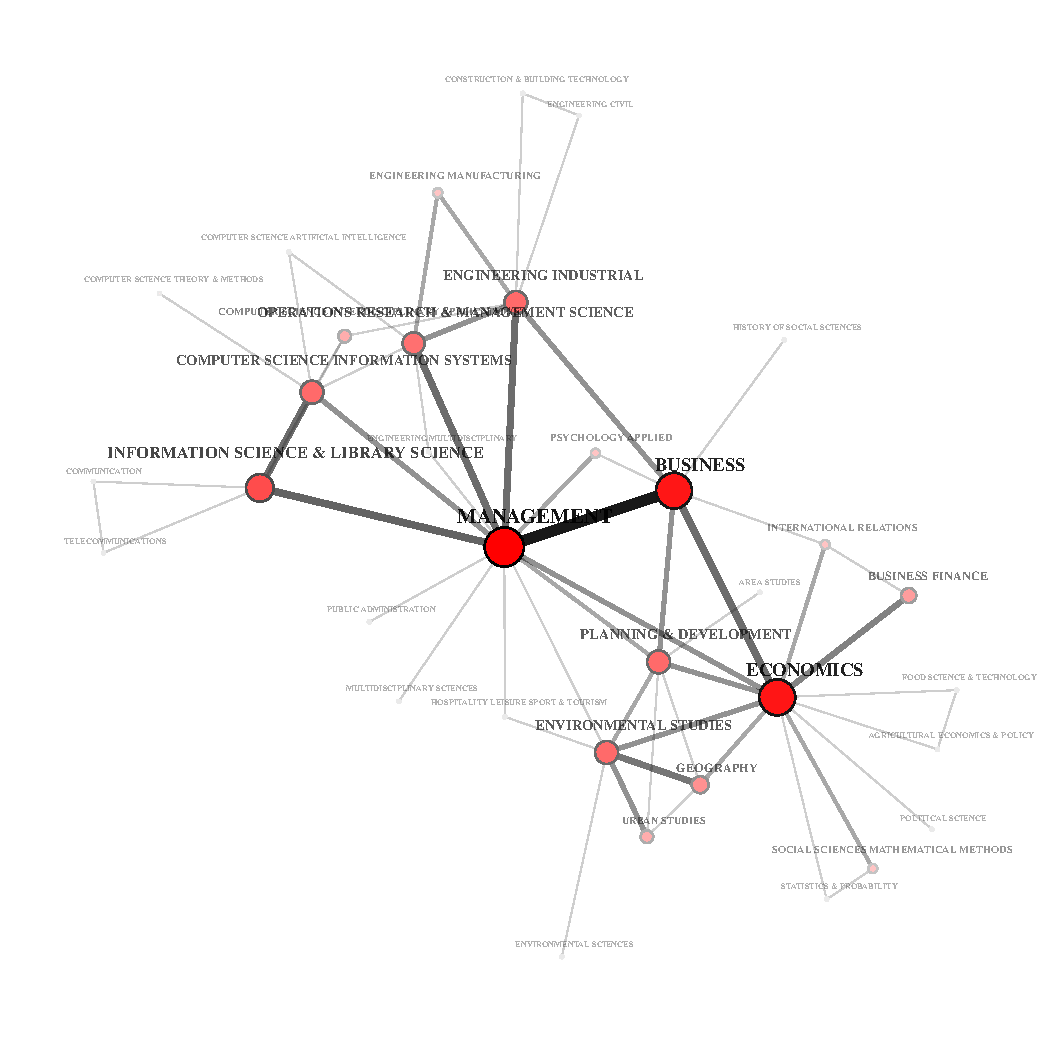
\includegraphics[width=1.5\textwidth]{report_files/bibx_report_net-categories.pdf}
}
\caption{Web of Science categories with most occurrences in unique sources}
\end{figure}

\clearpage

\begin{table}[htbp]
\centering
\caption{34 Web of Science categories with most occurrences in the sources, weighted by source count}
\makebox[\textwidth][c]{
\begin{tabular}{lrd{2}}
\toprule
\multicolumn{1}{l}{Name}&\multicolumn{1}{r}{Count}&\multicolumn{1}{r}{\%} \\
\midrule
Management & 196 & 32,13\\
Business & 125 & 20,49\\
Economics & 69 & 11,31\\
Engineering, industrial & 34 & 5,57\\
Planning \& development & 33 & 5,41\\
Information science \& library science & 28 & 4,59\\
Operations research \& management science & 27 & 4,43\\
Computer science, information systems & 16 & 2,62\\
Environmental studies & 15 & 2,46\\
Geography & 8 & 1,31\\
Multidisciplinary sciences & 7 & 1,15\\
Computer science, interdisciplinary applications & 6 & 0,98\\
Engineering, manufacturing & 5 & 0,82\\
Urban studies & 5 & 0,82\\
Business, finance & 4 & 0,66\\
Engineering, multidisciplinary & 4 & 0,66\\
Psychology, applied & 4 & 0,66\\
Social sciences, mathematical methods & 4 & 0,66\\
Statistics \& probability & 3 & 0,49\\
Environmental sciences & 2 & 0,33\\
International relations & 2 & 0,33\\
Agricultural economics \& policy & 1 & 0,16\\
Area studies & 1 & 0,16\\
Communication & 1 & 0,16\\
Computer science, artificial intelligence & 1 & 0,16\\
Computer science, theory \& methods & 1 & 0,16\\
Construction \& building technology & 1 & 0,16\\
Engineering, civil & 1 & 0,16\\
Food science \& technology & 1 & 0,16\\
History of social sciences & 1 & 0,16\\
Hospitality, leisure, sport \& tourism & 1 & 0,16\\
Political science & 1 & 0,16\\
Public administration & 1 & 0,16\\
Telecommunications & 1 & 0,16\\
Total & 610 & 100,00\\
\bottomrule
\multicolumn{3}{l}{\footnotesize Note: Sources can list multiple Web of Science categories} \\
\end{tabular}
}
\end{table}

\clearpage

\begin{figure}[p]
\makebox[\textwidth][c]{
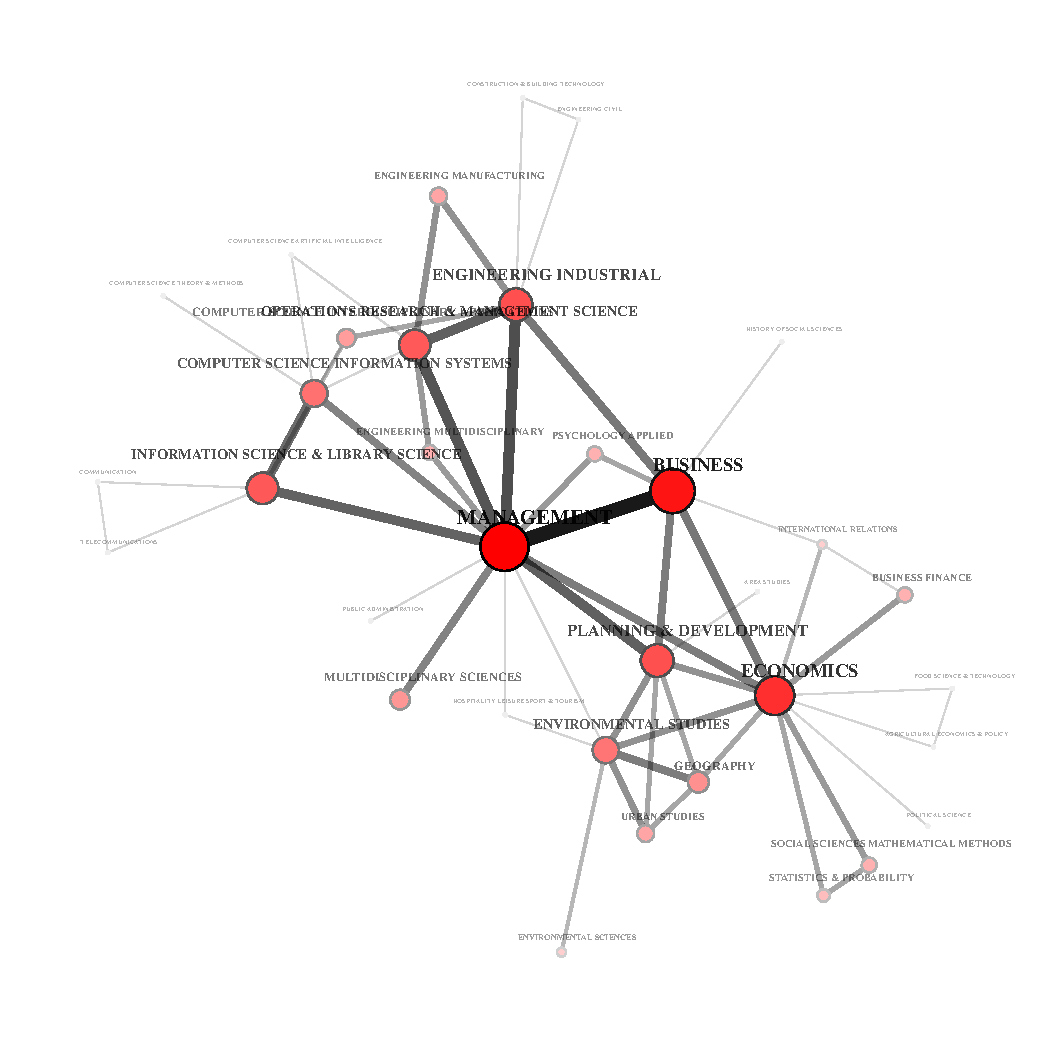
\includegraphics[width=1.5\textwidth]{report_files/bibx_report_net-categories-weighted.pdf}
}
\caption{Web of Science categories with most occurrences in the sources, weighted by source count}
\end{figure}

\clearpage

\begin{table}[htbp]
\centering
\caption{22 research areas with most occurrences in unique sources}
\makebox[\textwidth][c]{
\begin{tabular}{lrd{2}}
\toprule
\multicolumn{1}{l}{Name}&\multicolumn{1}{r}{Count}&\multicolumn{1}{r}{\%} \\
\midrule
Business \& economics & 124 & 56,62\\
Information science \& library science & 17 & 7,76\\
Computer science & 12 & 5,48\\
Engineering & 11 & 5,02\\
Public administration & 11 & 5,02\\
Environmental sciences \& ecology & 10 & 4,57\\
Operations research \& management science & 9 & 4,11\\
Geography & 5 & 2,28\\
Urban studies & 3 & 1,37\\
International relations & 2 & 0,91\\
Mathematical methods in social sciences & 2 & 0,91\\
Psychology & 2 & 0,91\\
Social sciences - other topics & 2 & 0,91\\
Agriculture & 1 & 0,46\\
Area studies & 1 & 0,46\\
Communication & 1 & 0,46\\
Construction \& building technology & 1 & 0,46\\
Food science \& technology & 1 & 0,46\\
Government \& law & 1 & 0,46\\
Mathematics & 1 & 0,46\\
Science \& technology - other topics & 1 & 0,46\\
Telecommunications & 1 & 0,46\\
Total & 219 & 100,00\\
\bottomrule
\multicolumn{3}{l}{\footnotesize Note: Sources can list multiple research areas} \\
\end{tabular}
}
\end{table}

\clearpage

\begin{figure}[p]
\makebox[\textwidth][c]{
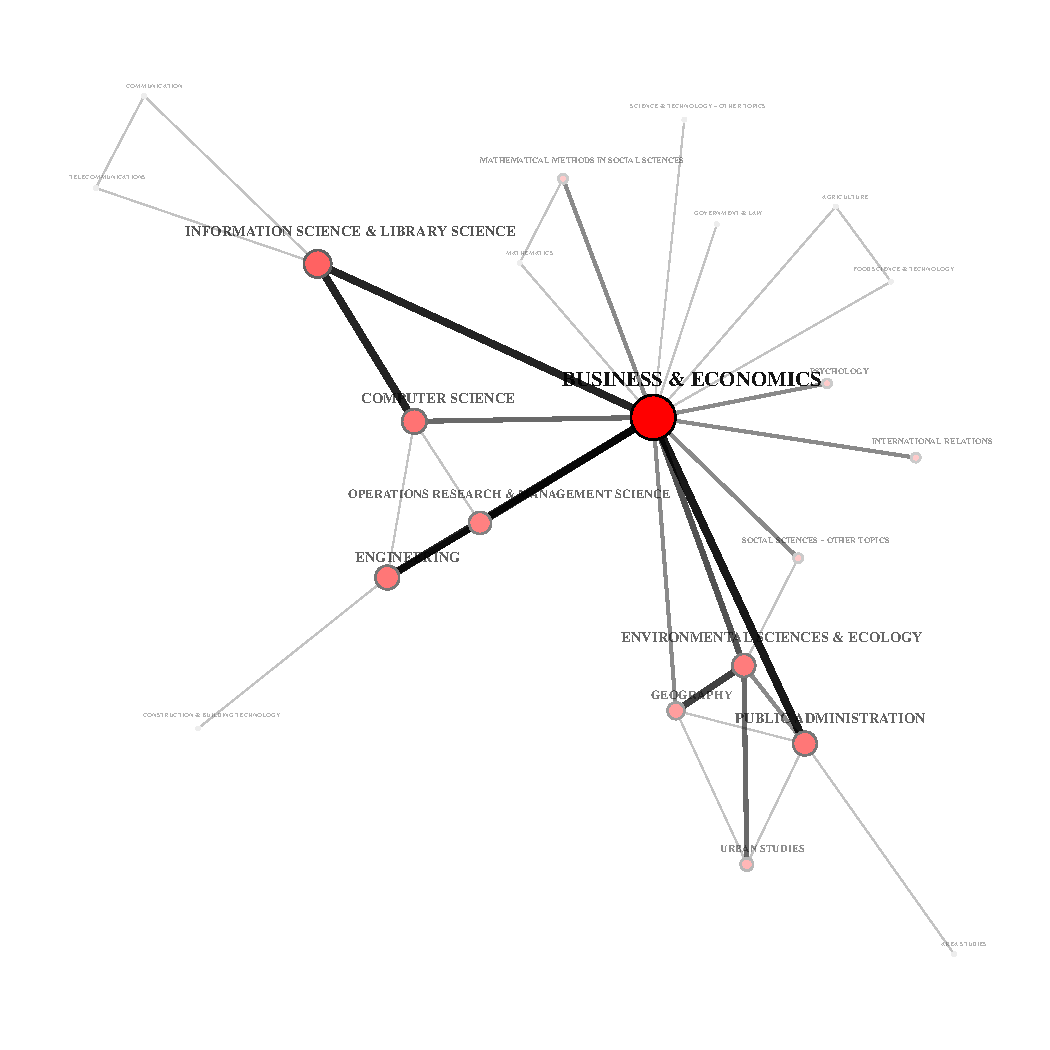
\includegraphics[width=1.5\textwidth]{report_files/bibx_report_net-areas.pdf}
}
\caption{Research areas with most occurrences in unique sources}
\end{figure}

\clearpage

\begin{table}[htbp]
\centering
\caption{22 research areas with most occurrences in the sources, weighted by source count}
\makebox[\textwidth][c]{
\begin{tabular}{lrd{2}}
\toprule
\multicolumn{1}{l}{Name}&\multicolumn{1}{r}{Count}&\multicolumn{1}{r}{\%} \\
\midrule
Business \& economics & 290 & 58,59\\
Engineering & 38 & 7,68\\
Public administration & 34 & 6,87\\
Information science \& library science & 28 & 5,66\\
Operations research \& management science & 27 & 5,45\\
Computer science & 21 & 4,24\\
Environmental sciences \& ecology & 15 & 3,03\\
Geography & 8 & 1,62\\
Science \& technology - other topics & 7 & 1,41\\
Urban studies & 5 & 1,01\\
Mathematical methods in social sciences & 4 & 0,81\\
Psychology & 4 & 0,81\\
Mathematics & 3 & 0,61\\
International relations & 2 & 0,40\\
Social sciences - other topics & 2 & 0,40\\
Agriculture & 1 & 0,20\\
Area studies & 1 & 0,20\\
Communication & 1 & 0,20\\
Construction \& building technology & 1 & 0,20\\
Food science \& technology & 1 & 0,20\\
Government \& law & 1 & 0,20\\
Telecommunications & 1 & 0,20\\
Total & 495 & 100,00\\
\bottomrule
\multicolumn{3}{l}{\footnotesize Note: Sources can list multiple research areas} \\
\end{tabular}
}
\end{table}

\clearpage

\begin{figure}[p]
\makebox[\textwidth][c]{
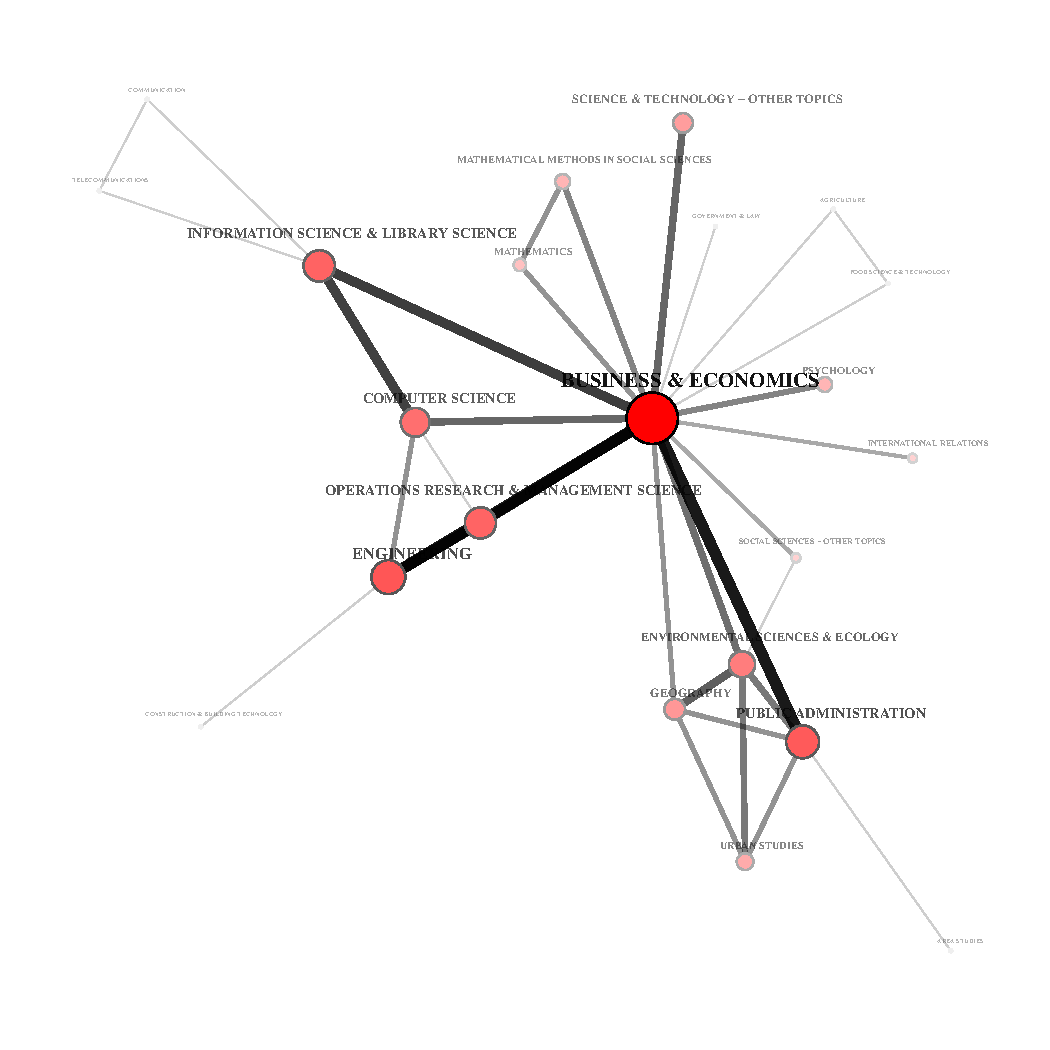
\includegraphics[width=1.5\textwidth]{report_files/bibx_report_net-areas-weighted.pdf}
}
\caption{Research areas with most occurrences in the sources, weighted by source count}
\end{figure}

\clearpage

\section{Keywords}

\begin{table}[H]
\centering
\caption{40 most mentioned author keywords}
\makebox[\textwidth][c]{
\begin{tabular}{lrd{2}}
\toprule
\multicolumn{1}{l}{Name}&\multicolumn{1}{r}{Count}&\multicolumn{1}{r}{\%} \\
\midrule
Absorptive capacity & 211 & 16,77\\
Innovation & 42 & 3,34\\
Knowledge management & 17 & 1,35\\
R\&d & 14 & 1,11\\
Organizational learning & 13 & 1,03\\
Knowledge & 11 & 0,87\\
Human capital & 9 & 0,72\\
Foreign direct investment & 8 & 0,64\\
Performance & 8 & 0,64\\
Dynamic capabilities & 7 & 0,56\\
Economic growth & 7 & 0,56\\
Knowledge transfer & 7 & 0,56\\
Open innovation & 7 & 0,56\\
Smes & 7 & 0,56\\
Cognitive distance & 6 & 0,48\\
Knowledge acquisition & 6 & 0,48\\
Productivity & 6 & 0,48\\
Social capital & 6 & 0,48\\
Alliances & 5 & 0,40\\
China & 5 & 0,40\\
Innovation performance & 5 & 0,40\\
Knowledge spillovers & 5 & 0,40\\
Learning & 5 & 0,40\\
Structural equation modeling & 5 & 0,40\\
Entrepreneurial orientation & 4 & 0,32\\
Innovation capability & 4 & 0,32\\
Networks & 4 & 0,32\\
New product development & 4 & 0,32\\
Patents & 4 & 0,32\\
Realised absorptive capacity & 4 & 0,32\\
Acquisitions & 3 & 0,24\\
Appropriability & 3 & 0,24\\
Corporate entrepreneurship & 3 & 0,24\\
Fdi & 3 & 0,24\\
Internationalization & 3 & 0,24\\
Knowledge spillover & 3 & 0,24\\
Korea & 3 & 0,24\\
Learning processes & 3 & 0,24\\
Marketing strategy & 3 & 0,24\\
Organizational culture & 3 & 0,24\\
... & & \\
Total & 1258 & 100,00\\
\bottomrule
\multicolumn{3}{l}{\footnotesize Note: Articles can list multiple author keywords} \\
\end{tabular}
}
\end{table}

\clearpage

\begin{figure}[p]
\makebox[\textwidth][c]{
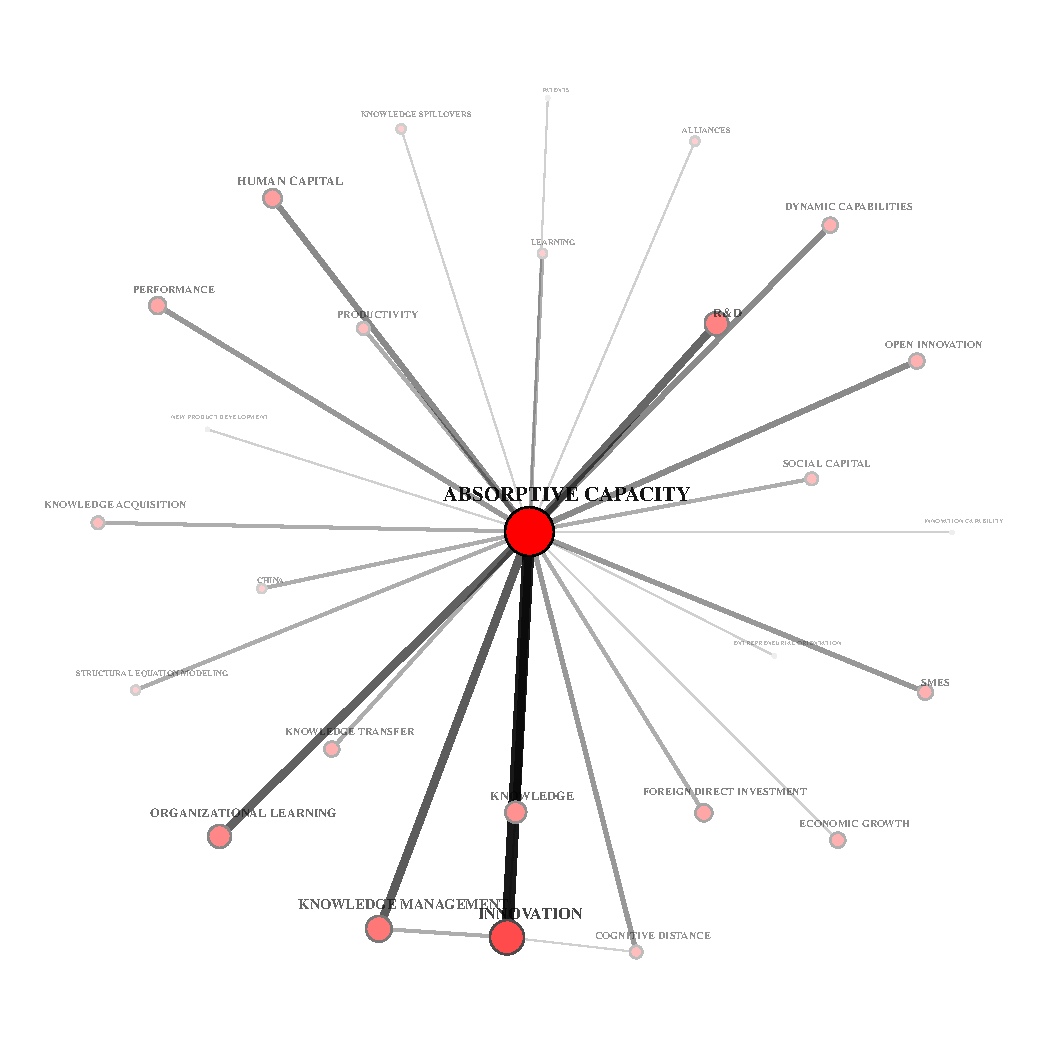
\includegraphics[width=1.5\textwidth]{report_files/bibx_report_net-keywords-author-relatedness.pdf}
}
\caption{Author keywords' relatedness (only keywords co-occurring 4 times or more shown)}
\end{figure}

\clearpage

\begin{table}[htbp]
\centering
\caption{40 most mentioned keywords plus}
\makebox[\textwidth][c]{
\begin{tabular}{lrd{2}}
\toprule
\multicolumn{1}{l}{Name}&\multicolumn{1}{r}{Count}&\multicolumn{1}{r}{\%} \\
\midrule
Innovation & 131 & 4,56\\
Performance & 100 & 3,48\\
Research-and-development & 80 & 2,78\\
Competitive advantage & 77 & 2,68\\
Perspective & 65 & 2,26\\
Knowledge & 59 & 2,05\\
Technology & 54 & 1,88\\
Firm & 53 & 1,84\\
Knowledge transfer & 52 & 1,81\\
Strategic alliances & 48 & 1,67\\
Dynamic capabilities & 46 & 1,60\\
Capabilities & 41 & 1,43\\
Product development & 41 & 1,43\\
Management & 39 & 1,36\\
Reconceptualization & 38 & 1,32\\
Firm performance & 35 & 1,22\\
Industry & 33 & 1,15\\
Firms & 32 & 1,11\\
Organizations & 28 & 0,97\\
Antecedents & 25 & 0,87\\
Networks & 24 & 0,84\\
Impact & 23 & 0,80\\
Model & 23 & 0,80\\
Resource-based view & 23 & 0,80\\
Productivity & 22 & 0,77\\
Spillovers & 22 & 0,77\\
Combinative capabilities & 21 & 0,73\\
Innovation performance & 19 & 0,66\\
Systems & 17 & 0,59\\
Joint ventures & 15 & 0,52\\
Market orientation & 15 & 0,52\\
Determinants & 14 & 0,49\\
Growth & 14 & 0,49\\
Technology-transfer & 14 & 0,49\\
Empirical-analysis & 13 & 0,45\\
Foreign direct-investment & 13 & 0,45\\
Information-technology & 12 & 0,42\\
International-joint-ventures & 12 & 0,42\\
Knowledge management & 12 & 0,42\\
Strategy & 11 & 0,38\\
... & & \\
Total & 2873 & 100,00\\
\bottomrule
\multicolumn{3}{l}{\footnotesize Note: Articles can list multiple keywords plus} \\
\end{tabular}
}
\end{table}

\clearpage

\begin{figure}[p]
\makebox[\textwidth][c]{
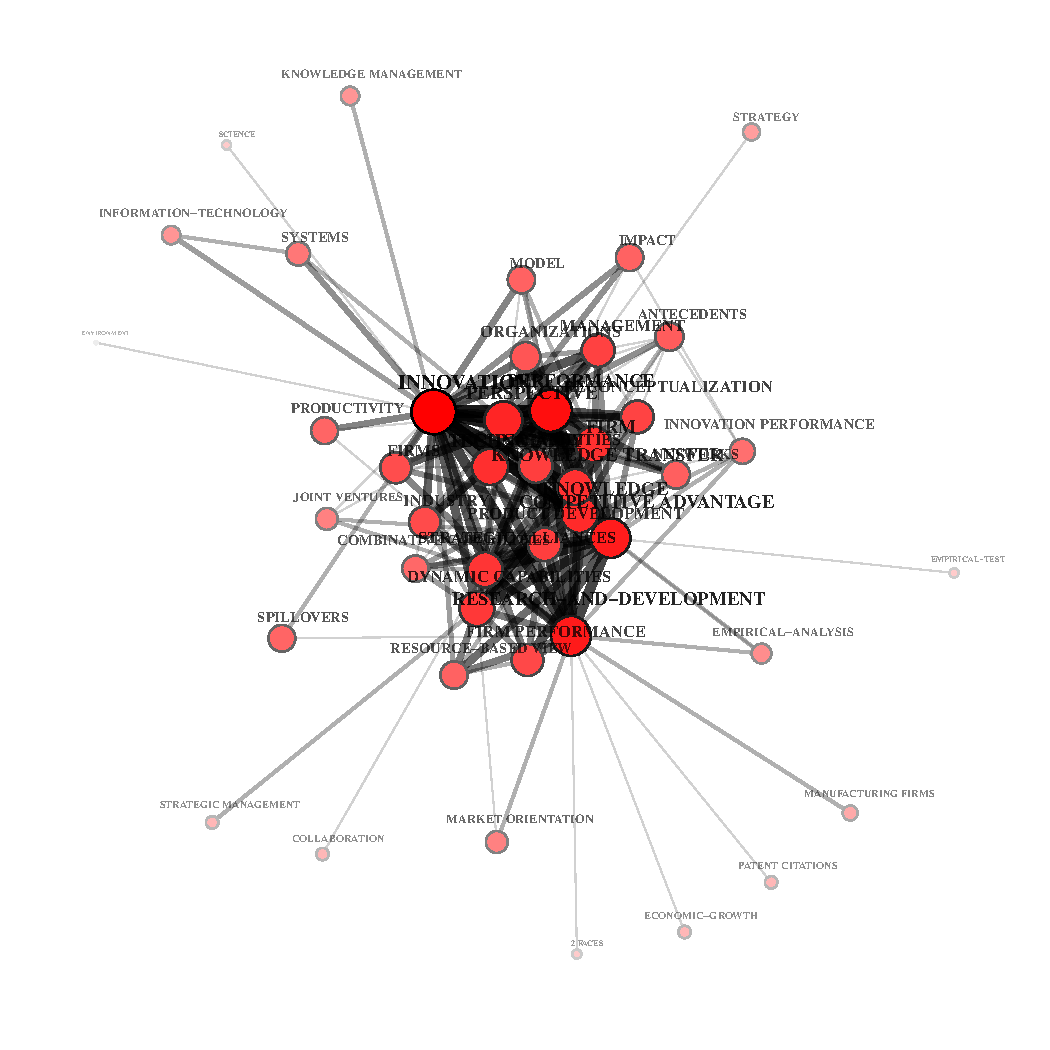
\includegraphics[width=1.5\textwidth]{report_files/bibx_report_net-keywords-plus-relatedness.pdf}
}
\caption{Keywords plus' relatedness (only keywords co-occurring 6 times or more shown)}
\end{figure}

\clearpage

\section{Cited references}

\begin{table}[H]
\centering
\caption{40 most cited references}
\makebox[\textwidth][c]{
\begin{tabular}{lrd{2}}
\toprule
\multicolumn{1}{l}{Name}&\multicolumn{1}{r}{Count}&\multicolumn{1}{r}{\%} \\
\midrule
COHEN WM, 1990, ADMIN SCI QUART, V35, P128 & 269 & 1,20\\
ZAHRA SA, 2002, ACAD MANAGE REV, V27, P185 & 223 & 1,00\\
LANE PJ, 1998, STRATEGIC MANAGE J, V19, P461 & 137 & 0,61\\
LANE PJ, 2006, ACAD MANAGE REV, V31, P833 & 124 & 0,55\\
COHEN WM, 1989, ECON J, V99, P569 & 113 & 0,51\\
JANSEN JJP, 2005, ACAD MANAGE J, V48, P999 & 99 & 0,44\\
SZULANSKI G, 1996, STRATEGIC MANAGE J, V17, P27 & 97 & 0,43\\
LANE PJ, 2001, STRATEGIC MANAGE J, V22, P1139 & 89 & 0,40\\
TODOROVA G, 2007, ACAD MANAGE REV, V32, P774 & 85 & 0,38\\
TSAI WP, 2001, ACAD MANAGE J, V44, P996 & 84 & 0,38\\
VAN DEN BOSCH FAJ, 1999, ORGAN SCI, V10, P551 & 71 & 0,32\\
VOLBERDA HW, 2010, ORGAN SCI, V21, P931 & 63 & 0,28\\
KOGUT B, 1992, ORGAN SCI, V3, P383 & 56 & 0,25\\
TEECE DJ, 1997, STRATEGIC MANAGE J, V18, P509 & 56 & 0,25\\
MOWERY DC, 1996, STRATEGIC MANAGE J, V17, P77 & 55 & 0,25\\
MARCH JG, 1991, ORGAN SCI, V2, P71 & 54 & 0,24\\
DYER JH, 1998, ACAD MANAGE REV, V23, P660 & 50 & 0,22\\
LICHTENTHALER U, 2009, ACAD MANAGE J, V52, P822 & 49 & 0,22\\
KIM L, 1998, ORGAN SCI, V9, P506 & 47 & 0,21\\
GRANT RM, 1996, STRATEGIC MANAGE J, V17, P109 & 46 & 0,21\\
PODSAKOFF PM, 2003, J APPL PSYCHOL, V88, P879 & 45 & 0,20\\
COCKBURN IM, 1998, J IND ECON, V46, P157 & 44 & 0,20\\
EISENHARDT KM, 2000, STRATEGIC MANAGE J, V21, P1105 & 44 & 0,20\\
HUBER GP, 1991, ORGAN SCI, V2, P88 & 43 & 0,19\\
NONAKA I., 1995, KNOWLEDGE CREATING C & 43 & 0,19\\
BARNEY J, 1991, J MANAGE, V17, P99 & 42 & 0,19\\
NELSON R. R., 1982, EVOLUTIONARY THEORY & 40 & 0,18\\
COHEN WM, 1994, MANAGE SCI, V40, P227 & 39 & 0,17\\
LENOX M, 2004, STRATEGIC MANAGE J, V25, P331 & 38 & 0,17\\
FOSFURI A, 2008, OMEGA-INT J MANAGE S, V36, P173 & 37 & 0,17\\
FORNELL C, 1981, J MARKETING RES, V18, P39 & 36 & 0,16\\
STOCK G.N., 2001, J HIGH TECHNOLOGY MA, V12, P77 & 35 & 0,16\\
LAURSEN K, 2006, STRATEGIC MANAGE J, V27, P131 & 34 & 0,15\\
VEUGELERS R, 1997, RES POLICY, V26, P303 & 34 & 0,15\\
CHESBROUGH H. W., 2003, OPEN INNOVATION NEW & 32 & 0,14\\
LEVINTHAL DA, 1993, STRATEGIC MANAGE J, V14, P95 & 32 & 0,14\\
POWELL WW, 1996, ADMIN SCI QUART, V41, P116 & 32 & 0,14\\
ESCRIBANO A, 2009, RES POLICY, V38, P96 & 31 & 0,14\\
GUPTA AK, 2000, STRATEGIC MANAGE J, V21, P473 & 30 & 0,13\\
NONAKA I, 1994, ORGAN SCI, V5, P14 & 29 & 0,13\\
... & & \\
Total & 22367 & 100,00\\
\bottomrule
\multicolumn{3}{l}{\footnotesize } \\
\end{tabular}
}
\end{table}

\clearpage

\begin{table}[htbp]
\centering
\caption{40 most recent years cited}
\makebox[\textwidth][c]{
\begin{tabular}{lrd{2}}
\toprule
\multicolumn{1}{l}{Year}&\multicolumn{1}{r}{Count}&\multicolumn{1}{r}{\%} \\
\midrule
2015 & 30 & 0,13\\
2014 & 110 & 0,49\\
2013 & 237 & 1,06\\
2012 & 395 & 1,77\\
2011 & 589 & 2,63\\
2010 & 742 & 3,32\\
2009 & 854 & 3,82\\
2008 & 873 & 3,90\\
2007 & 1035 & 4,63\\
2006 & 1153 & 5,15\\
2005 & 1162 & 5,20\\
2004 & 1071 & 4,79\\
2003 & 1160 & 5,19\\
2002 & 1152 & 5,15\\
2001 & 1213 & 5,42\\
2000 & 1020 & 4,56\\
1999 & 869 & 3,89\\
1998 & 1054 & 4,71\\
1997 & 655 & 2,93\\
1996 & 916 & 4,10\\
1995 & 622 & 2,78\\
1994 & 612 & 2,74\\
1993 & 430 & 1,92\\
1992 & 417 & 1,86\\
1991 & 528 & 2,36\\
1990 & 633 & 2,83\\
1989 & 348 & 1,56\\
1988 & 312 & 1,39\\
1987 & 141 & 0,63\\
1986 & 236 & 1,06\\
1985 & 155 & 0,69\\
1984 & 170 & 0,76\\
1983 & 103 & 0,46\\
1982 & 157 & 0,70\\
1981 & 136 & 0,61\\
1980 & 88 & 0,39\\
1979 & 82 & 0,37\\
1978 & 83 & 0,37\\
1977 & 115 & 0,51\\
1976 & 42 & 0,19\\
... & & \\
Total & 22367 & 100,00\\
\bottomrule
\multicolumn{3}{p{3.75cm}}{\footnotesize Note: Some references do not\newline contain year information} \\
\end{tabular}
}
\end{table}

\clearpage

\begin{table}[htbp]
\centering
\caption{40 most cited authors}
\makebox[\textwidth][c]{
\begin{tabular}{lrd{2}}
\toprule
\multicolumn{1}{l}{Name}&\multicolumn{1}{r}{Count}&\multicolumn{1}{r}{\%} \\
\midrule
COHEN WM & 439 & 1,96\\
LANE PJ & 356 & 1,59\\
ZAHRA SA & 301 & 1,35\\
JANSEN JJP & 117 & 0,52\\
TSAI WP & 117 & 0,52\\
SZULANSKI G & 111 & 0,50\\
TEECE DJ & 111 & 0,50\\
KOGUT B & 104 & 0,46\\
MOWERY DC & 102 & 0,46\\
GRANT RM & 96 & 0,43\\
TODOROVA G & 86 & 0,38\\
EISENHARDT KM & 84 & 0,38\\
LICHTENTHALER U & 83 & 0,37\\
VOLBERDA HW & 77 & 0,34\\
DYER JH & 75 & 0,34\\
VAN DEN BOSCH FAJ & 73 & 0,33\\
PODSAKOFF PM & 72 & 0,32\\
{[}ANONYMOUS{]} & 71 & 0,32\\
MARCH JG & 68 & 0,30\\
ROTHAERMEL FT & 60 & 0,27\\
AHUJA G & 59 & 0,26\\
CASSIMAN B & 59 & 0,26\\
JAFFE AB & 56 & 0,25\\
ARGOTE L & 53 & 0,24\\
NELSON R. R. & 53 & 0,24\\
NONAKA I. & 52 & 0,23\\
GUPTA AK & 51 & 0,23\\
KIM L & 51 & 0,23\\
NONAKA I & 51 & 0,23\\
HUBER GP & 50 & 0,22\\
VEUGELERS R & 49 & 0,22\\
COCKBURN IM & 47 & 0,21\\
FORNELL C & 47 & 0,21\\
FOSFURI A & 47 & 0,21\\
BARNEY J & 46 & 0,21\\
LAURSEN K & 46 & 0,21\\
TUSHMAN ML & 45 & 0,20\\
GULATI R & 44 & 0,20\\
POWELL WW & 44 & 0,20\\
CHESBROUGH H. W. & 43 & 0,19\\
... & & \\
Total & 22367 & 100,00\\
\bottomrule
\multicolumn{3}{l}{\footnotesize Note: Some references do not contain author information} \\
\end{tabular}
}
\end{table}

\clearpage

\begin{figure}[p]
\makebox[\textwidth][c]{
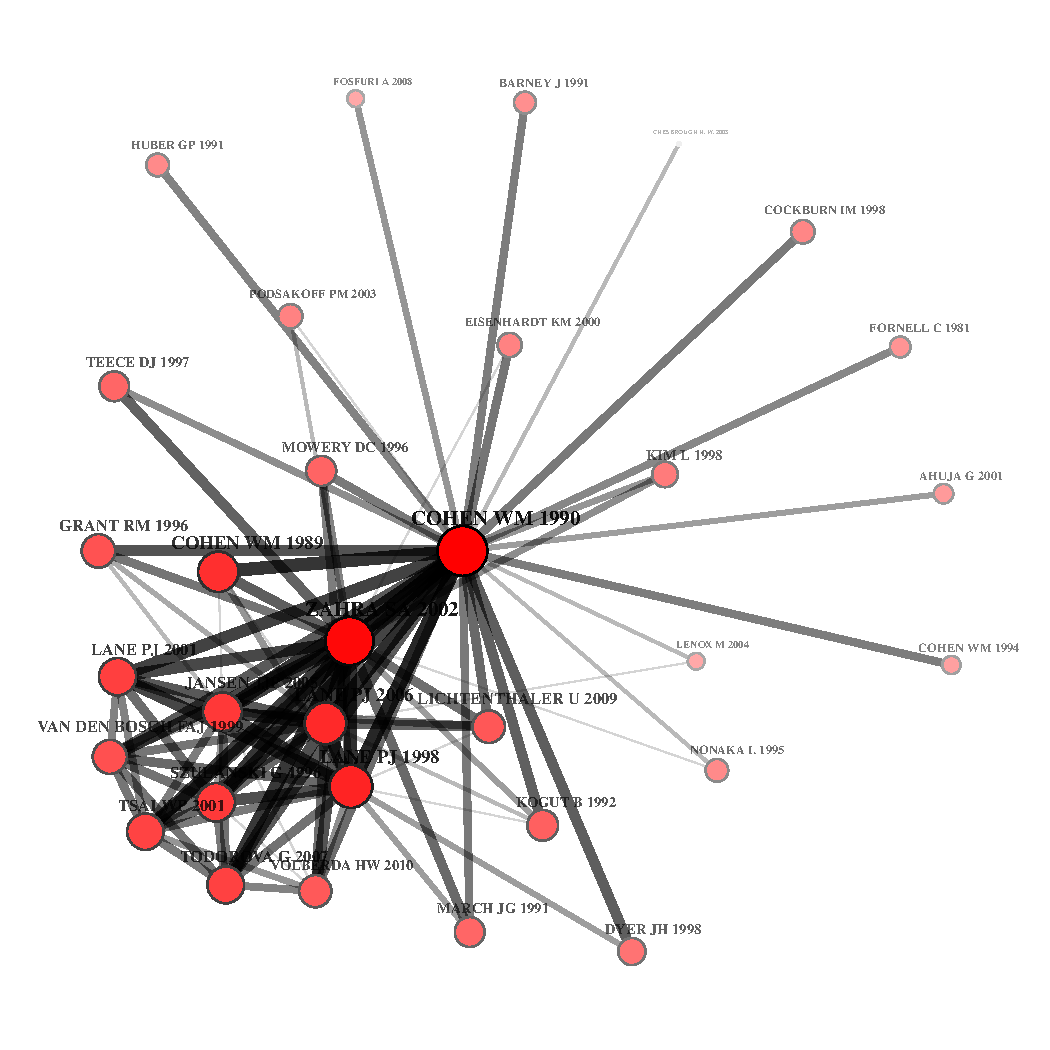
\includegraphics[width=1.5\textwidth]{report_files/bibx_report_net-cocitations.pdf}
}
\caption{Cocitation network (only cocitations recurring 30 times or more shown)}
\end{figure}

\clearpage

\setcounter{secnumdepth}{0}
\addtocontents{toc}{\vspace{\normalbaselineskip} \vspace{\normalbaselineskip} \bfseries Appendices\par}

{\centering
\vspace*{\fill}
{\huge \bfseries Appendices\par}
\rule{0pt}{10ex}
\vspace*{\fill}
} % centering
\thispagestyle{empty}
\clearpage

\begin{multicols*}{3}
[
\section{Appendix: All authors}
List all authors for WoS data inconsistency inspection, suspects highlighted.
]
\begin{footnotesize}
Abareshi, A \\ Abecassis-Moedas, C \\ Abreu, MA \\ Acs, ZJ \\ Adams, D \\ Ahlin, B \\ Ahlstrom, D \\ Akbar, H \\ Al-Dajani, H \\ Albors-Garrigos, J \\ Alegre, J \\ Alexander, A \\ Alexandre, MT \\ Allen, MW \\ Ambrosini, V \\ Anand, J \\ Andersen, J \\ Anderson, MH \\ Antonacopoulou, E \\ Anwar, S \\ Aranguren, M \\ Arbussa, A \\ Archontakis, F \\ Arias-Aranda, D \\ Aribi, A \\ Ariza-Montes, JA \\ Armbruster, H \\ Armstrong, DJ \\ Arnold, V \\ Augier, P \\ Azadegan, A \\ Azagra-Caro, JM \\ Bachor, V \\ Backmann, J \\ Bagchi-Sen, S \\ Balan-Vnuk, E \\ Bao, Q \\ Barbosa, N \\ Becker, SO \\ Becker-Ritterspach, F \\ Beckett, RC \\ Belcher, SM \\ Belderbos, R \\ Bell, J \\ Ben Mahmoud-Jouini, S \\ Ben-Menahem, SM \\ Ben-Oz, C \\ Benford, T \\ Bergeron, F \\ Berges-Muro, L \\ Bergh, DD \\ Bertrand, O \\ Bharadwaj, S \\ Bharati, P \\ Bishop, K \\ Bjorkman, I \\ Blind, K \\ Blomqvist, K \\ Bodman, P \\ Bogers, M \\ Bolivar-Ramos, MT \\ Boyd, B \\ Brandon-Jones, A \\ Brettel, M \\ Breunig, KJ \\ Brown, V \\ Bruni, M \\ Buckley, PJ \\ Burcharth, ALLD \\ Bustinza, OF \\ Cadot, O \\ Calero-Medina, C \\ Camacho, J \\ Camison, C \\ Campisi, D \\ Cao, M \\ Capo-Vicedo, J \\ Caragliu, A \\ Cardenas, J \\ Casali, GL \\ Castellacci, F \\ Catozzella, A \\ Cavusgil, ST \\ Cegarra-Navarro, JG \\ Cepeda-Carrion, G \\ Chalmers, DM \\ Chang, CC \\ Chang, CH \\ Chang, CW \\ Chang, S \\ \hl{Chang, SF} \\ Chang, YY \\ Chatterji, M \\ Chaudhury, A \\ Chen, CC \\ Chen, CJ \\ Chen, CLJ \\ Chen, JS \\ Chen, YS \\ Cheng, DJ \\ Chin, WW \\ Cho, SW \\ Choi, S \\ Chou, SW \\ Chuang, YS \\ Chung, MY \\ Cieslik, A \\ Clarysse, B \\ Clausen, TH \\ Coccia, M \\ Cockburn, IM \\ Coenders, G \\ COHEN, WM \\ Cordery, JL \\ Correani, L \\ Croteau, AM \\ Cuellar, MJ \\ D'Este, P \\ D'Oria, L \\ D'Souza, DE \\ Dai, M \\ Daniel, EM \\ Davids, M \\ de Boer, M \\ de Groot, HLF \\ de Jong, JPJ \\ de Renzio, P \\ de Silva, A \\ De-Miguel, B \\ Debrulle, J \\ Deeds, DL \\ Delmas, M \\ Deng, XD \\ Denicolai, S \\ Di Gangi, PM \\ Dinger, M \\ Dobrzykowski, DD \\ Doll, WJ \\ Dovis, M \\ Dreher, C \\ Drnovsek, M \\ Dupouet, O \\ Durham, JB \\ Durisin, B \\ Dutta, S \\ Duysters, G \\ Easterby-Smith, M \\ Ebers, M \\ Egbetokun, A \\ Egger, PH \\ Eiriz, V \\ El Sawy, OA \\ Eldridge, S \\ Elmawazini, K \\ Elola, A \\ Engelen, A \\ Enkel, E \\ Eren, M \\ Escribano, A \\ Exposito-Langa, M \\ Fabrizio, KR \\ Falvey, R \\ Feeny, S \\ Fei, WC \\ Feng, YQ \\ Ferdinand, J \\ Fernandez-de-Lucio I \\ Fernandez-De-Lucio, I \\ Fernandez-Mesa, A \\ Fernhaber, SA \\ Ferragina, AM \\ Ferreras-Mendez, JL \\ Fey, CF \\ Fiegenbaum, A \\ Filatotchev, I \\ Flaten, BT \\ Flatten, T \\ \hl{Flatten, TC} \\ Flor, ML \\ Fores, B \\ Fosfuri, A \\ Foss, NJ \\ Foster, N \\ Foster-McGregor, N \\ Francalanci, C \\ Franco, C \\ Freel, M \\ Galbraith, B \\ Gallivan, MJ \\ Galluch, PS \\ Gao, SX \\ Garcia-Morales, VJ \\ Garcia-Vazquez, JM \\ Garcia-Villaverde, PM \\ Garofalo, G \\ Gauch, S \\ Gebauer, H \\ Gellynck, X \\ George, G \\ Ghimire, A \\ Gilsing, V \\ \hl{Gilsing, VA} \\ Giovacchini, E \\ Girma, S \\ Giuliani, E \\ Glas, A \\ Gnyawali, DR \\ Gomez, J \\ Gong, YP \\ Gopinath, M \\ Gosain, S \\ Graca, M \\ Gray, C \\ Greenaway, D \\ Greve, GI \\ Greve, HR \\ Griffith, R \\ Grimpe, C \\ Grover, V \\ Grunfeld, LA \\ Gunawan, J \\ Guo, B \\ Guo, HF \\ Gutierrez, LJG \\ Gutierrez-Gracia, A \\ Guttel, W \\ Hagemeister, M \\ Hagemejer, J \\ Hall, KD \\ Halmenschlager, C \\ Hammerschmidt, A \\ Hampton, C \\ Han, Y \\ Harmaakorpi, V \\ Haro-Dominguez, MD \\ Harris, R \\ Harvey, G \\ Hasan, I \\ Hatfield, DE \\ Hayton, JC \\ He, XM \\ Heeley, MB \\ Heil, S \\ Henderson, RM \\ Hernandez-Perlines, F \\ Hervas-Oliver, JL \\ Hidalgo, A \\ Hisrich, RD \\ Hobday, M \\ Hoegl, M \\ Hoffmann, VH \\ Hollensen, S \\ Hong, PC \\ Hotho, JJ \\ Hsu, CC \\ Hu, DC \\ Hu, Q \\ Hua, ZS \\ Huang, F \\ Huang, IC \\ Huang, KF \\ Hubler, M \\ Hughes, B \\ Hughes, M \\ Hughes, P \\ Hung, CH \\ Huo, JG \\ Hur, YS \\ Hurmelinna-Laukkanen, P \\ Hussinger, K \\ Intindola, M \\ Ioannou, G \\ Ireland, RD \\ Isaksson, A \\ Ismail, HS \\ Iyengar, K \\ Jacobson, D \\ Jaime, A \\ Jansen, JJP \\ Jas, P \\ Javalgi, RG \\ Jia, LD \\ Jiang, CX \\ Jimenez-Barrionuevo, MM \\ Jimenez-Castillo, D \\ Jimenez-Jimenez, D \\ Johnston, DA \\ Johnston, WJ \\ Jones, O \\ Jordaan, JA \\ Joshi, K \\ Jung-Erceg, P \\ Kaiser, U \\ Kallio, A \\ Kamien, MI \\ Kask, J \\ Kaulich, F \\ Kauppi, K \\ Ke, WL \\ Keil, T \\ Keller, RT \\ Keller, W \\ Khwaja, AI \\ Kim, B \\ Kim, E \\ Kim, M \\ Kim, YA \\ King, A \\ Kneller, R \\ Knockaert, M \\ Knoppen, D \\ Knott, AM \\ Kodama, T \\ Kohtamaki, M \\ Kok, RAW \\ Koka, BR \\ Kostopoulos, K \\ Kotabe, M \\ Kovacic, A \\ Kube, H \\ Kulkarni, SS \\ Kuss, M \\ \hl{Kuss, MJ} \\ Kwee, Z \\ Lai, MY \\ Lan, PN \\ Lane, PJ \\ Larraneta, B \\ Lau, AKW \\ Lazaric, N \\ Le, T \\ Leahy, D \\ Leal-Millan, A \\ \hl{Leal-Millan, AG} \\ Leal-Rodriguez, AL \\ Lee, CY \\ Lee, DS \\ Lee, ES \\ Lee, H \\ Lee, J \\ \hl{Lee, JS} \\ Lee, K \\ \hl{Lee, KC} \\ Lee, SC \\ Lenox, M \\ Lettl, C \\ Leuschner, R \\ Lev, S \\ Levi-Jaksic, M \\ LEVINTHAL, DA \\ Lewin, AY \\ Lhuillery, S \\ Li, D \\ Li, HY \\ Li, J \\ Li, QC \\ Li, XB \\ Li, Y \\ Liang, HG \\ Liang, HM \\ Liao, JW \\ Liao, SH \\ Liao, TJ \\ Lichtenthaler, E \\ Lichtenthaler, U \\ Lim, ENK \\ Lim, K \\ Lima, V \\ Lin, BW \\ Lin, CH \\ Lin, CY \\ Lin, HL \\ Lin, KH \\ Lin, MJJ \\ Lin, YH \\ Liu, CY \\ Liu, HF \\ Liu, LN \\ Liu, XF \\ Llorens-Montes, FJ \\ Lo, W \\ Longhi, C \\ Lopez, S \\ Love, JH \\ Lu, IY \\ Lubatkin, M \\ Luo, JL \\ Lyles, MA \\ Maes, J \\ Makinen, SJ \\ Malhotra, A \\ Malipiero, A \\ Mancusi, ML \\ Mancuso, P \\ Manfreda, A \\ Manga, P \\ Marabelli, M \\ Marcin, K \\ Mariano, S \\ Martin, N \\ Martin-de Castro, G \\ Martin-Rojas, R \\ Martinez, H \\ Martinez-Caro, E \\ Martinez-Sanchez, A \\ Martinez-Senra, AI \\ Martinkenaite, I \\ Marzucchi, A \\ Massini, S \\ Matthyssens, P \\ Mattsson, P \\ Matusik, SF \\ Maula, M \\ Maurer, I \\ Mazzotta, F \\ McAdam, M \\ McAdam, R \\ Mcgillivray, M \\ Melkas, H \\ Mian, A \\ Miguelez, E \\ Miller, K \\ Minbaeva, D \\ \hl{Minbaeva, DB} \\ Moffett, S \\ Moilanen, M \\ Mol, MJ \\ Molina, LM \\ Molina, VB \\ Molina-Morales, FX \\ Molla, A \\ Montagna, C \\ Montealegre, R \\ Montresor, S \\ Morabito, V \\ Moreno, AR \\ Moreno, R \\ Moreno-Garcia, J \\ Morgan, RE \\ Moutinho, RFF \\ Mukherji, N \\ Muller-Seitz, G \\ Munari, F \\ Murovec, N \\ Murray, JY \\ Nagati, H \\ Naghavi, A \\ Najmi, M \\ Narasimhan, O \\ Nastasi, A \\ Natera, JM \\ Natti, S \\ Navarro, JGC \\ Neary, JP \\ Neely, A \\ Nemanich, LA \\ Newell, S \\ Newey, L \\ \hl{Newey, LR} \\ Nguyen, B \\ Nicotra, M \\ Nieto, M \\ Nijkamp, P \\ Noblet, JP \\ Nooteboom, B \\ Noyons, ECM \\ Nunnenkamp, P \\ Olander, H \\ Oltra, MJ \\ Ooms, W \\ Ostbye, S \\ Ouyang, HW \\ Paff, LA \\ Pai, DC \\ Pak, MS \\ Pandza, K \\ Panfilii, V \\ Papachroni, M \\ Papalexandris, A \\ Parada, MJ \\ Parent, R \\ Parida, V \\ Parjanen, S \\ Park, BI \\ Park, HJ \\ Park, JG \\ Park, JH \\ Parra-Requena, G \\ Pastorino, N \\ Patel, PC \\ Pathak, S \\ Patterson, W \\ Patton, D \\ Pauwels, P \\ Pedersen, T \\ Peeters, C \\ Peltola, T \\ Peng, MW \\ Peng, SJ \\ Perruchas, F \\ Phan, PH \\ Pieniak, Z \\ Pihkala, T \\ Pinkse, J \\ Pittz, TG \\ Popaitoon, S \\ Posen, HE \\ Powell, A \\ Prodan, I \\ Pugliesi, S \\ Puthusserry, P \\ Qi, GY \\ Qian, HF \\ Quevedo, P \\ Quintas, MA \\ Radojicic, Z \\ Radovanovic, N \\ Ragu-Nathan, TS \\ Rajiv, S \\ Ramirez, M \\ Ranguelov, S \\ Raymond, L \\ Rebolledo, C \\ Redding, S \\ Reid, MF \\ Revilla, E \\ Rice, J \\ Riemenschneider, CK \\ Ritala, P \\ Roberts, N \\ Robertson, PL \\ Rodriguez-Castellanos, A \\ Roh, JJ \\ Roldan, JL \\ Romano, M \\ Ronchi, S \\ Roper, S \\ Rose, EL \\ Rosell-Martinez, J \\ Rothaermel, FT \\ Ruiz-Moreno, A \\ Ruiz-Ortega, MJ \\ Saadi, S \\ Saenz, MJ \\ Saito, H \\ Saka-Helmhout, A \\ Salk, JE \\ Sanchez-Perez, M \\ Sanchez-Sellero, P \\ Saraf, N \\ Sartal, A \\ Savin, I \\ Schildt, H \\ Schillaci, CE \\ Schleimer, SC \\ Schmidt, S \\ Sciascia, S \\ Scott, JT \\ Sels, L \\ Seo, YW \\ Setia, P \\ Sharifi, H \\ Sharkey, TW \\ Sharma, S \\ Shoham, A \\ Shulman, AD \\ Siengthai, S \\ Silberman, J \\ Simon, E \\ Skelcher, C \\ Smit, MJ \\ Smith, HL \\ Sobrero, M \\ Sofka, W \\ Soleimanof, S \\ Song, DW \\ Song, J \\ Song, ZH \\ Spencer, E \\ Spithoven, A \\ Srivastava, MK \\ St-Pierre, J \\ Stahl, GK \\ Stemberger, MI \\ Stevens, PA \\ Stoica, M \\ Su, TH \\ Su, ZF \\ Sugheir, J \\ Suh, HJ \\ Sun, PYT \\ Sun, Y \\ Sutton, SG \\ Suzuki, S \\ Sweeney, JR \\ Tai, SYTT \\ Tan, BR \\ Tang, YK \\ Tapia, AH \\ Tavani, SN \\ Taylor, JE \\ Techatassanasoontorn, AA \\ Teigland, R \\ Terjesen, S \\ Thomas, C \\ Thomas, R \\ Tidd, J \\ Todorova, G \\ Tomas-Miquel, JV \\ Tortoriello, M \\ Tribo, JA \\ Trkman, P \\ Truffer, B \\ Tsai, WP \\ Tsai, Y \\ \hl{Tsai, YC} \\ Tseng, CY \\ Tsui, KA \\ Tu, Q \\ Turpin, T \\ Tzokas, N \\ Ulhoi, JP \\ Unsal, HI \\ Uotila, T \\ Vaara, E \\ Valdaliso, J \\ Van den Bosch, FAJ \\ van den Oord, A \\ Van Haverbeke, W \\ van Raaij, EM \\ Van Reenen, J \\ Vandenbempt, K \\ Vargas, P \\ Vasudeva, G \\ Vazquez, XH \\ Vega-Jurado, J \\ Vera, D \\ Verbeke, A \\ Verbeke, W \\ Verreynne, ML \\ Vicente-Oliva, S \\ Vilkko, MK \\ Vivarelli, M \\ Volberda, HW \\ von Ehrlich, M \\ Vonderembse, MA \\ Voss, H \\ Wales, WJ \\ Walshe, K \\ Walter, A \\ Walter, C \\ Wan, DF \\ Wang, CF \\ Wang, TN \\ Wang, WH \\ Wang, WW \\ Wang, YQ \\ Wareham, J \\ Watkins, TA \\ Way, SA \\ Wei, KK \\ Wei, YQ \\ Welsch, H \\ Wensley, AKP \\ Wiethaus, L \\ Wincent, J \\ Winkelbach, A \\ Woll, K \\ Woo, H \\ Wood, E \\ Worch, H \\ Wright, M \\ Wu, AQ \\ Wu, CC \\ Wu, CS \\ Wu, JY \\ Wu, LY \\ Wu, XB \\ Wu, YJ \\ Xia, TJ \\ Xie, XM \\ Xiong, GY \\ Xu, H \\ Xu, K \\ Xue, YJ \\ Yanez-Araque, B \\ Yang, CH \\ Yang, HD \\ Yang, JJ \\ Yasar, M \\ Yu, CM \\ Yu, MJ \\ Yu, PH \\ Zahra, SA \\ Zang, I \\ Zhang, C \\ Zhang, KH \\ Zhang, M \\ Zhang, Y \\ Zhao, XD \\ Zhou, J \\ Zhou, LA \\ Zhu, KX \\ Zhuang, H \\ Zia, B
\end{footnotesize}
\end{multicols*}

\clearpage

\begin{multicols*}{2}
[
\section{Appendix: All parsed institutions}
List all parsed institutions for WoS data inconsistency inspection, suspects highlighted.
]
\begin{footnotesize}
Aachen Univ RWTH \\ Aalto Univ \\ Aarhus Univ \\ Acad Gen Mil \\ Aix Marseille Univ \\ Arizona State Univ \\ Asian Inst Technol \\ Aston Univ \\ Athens Univ Econ \& Business \\ Australian Natl Univ \\ Avison Consulting Ltd \\ BI Norwegian Business Sch \\ Babson Coll \\ Ball State Univ \\ Bangkok Univ \\ Baylor Univ \\ Belgian Sci Policy \\ Bentley Univ \\ Birkbeck \\ Bloomsburg Univ Penn \\ Bocconi Univ \\ Boise State Univ \\ Boston Consulting Grp Inc \\ Bournemouth Univ \\ Bryant Univ \\ Butler Univ \\ CESifo \\ CNRS \\ CSIC UPV \\ CUNEF Business Sch \\ Cardiff Univ \\ Carnegie Mellon Univ \\ Case Western Reserve Univ \\ Catholic Univ Leuven \\ Catholic Univ Louvain \\ Catholic Univ Milan \\ China Europe Int Business Sch \\ Chinese Univ Hong Kong \\ Chonnam Natl Univ \\ Chungchou Inst Technol \\ City Univ Hong Kong \\ City Univ London \\ Clarkson Univ \\ Clemson Univ \\ Cleveland State Univ \\ Coll Carlo Alberto \\ Colorado Sch Mines \\ Colorado State Univ \\ Columbia Univ \\ Commerce Dev Res Inst \\ Commites \\ Concordia Univ \\ Consumer \& Sensory Res Inst \\ Copenhagen Business Sch \\ Copenhagen Sch Econ \& Business Adm \\ Cornell Univ \\ Ctr European Econ Res \\ Ctr Univ Def \\ Curtin Univ \\ Dartmouth Coll \\ Delft Univ Technol \\ Depaul Univ \\ Dept Strategy \& Management \\ Dublin City Univ \\ Duke Univ \\ E Carolina Univ \\ E China Univ Sci \& Technol \\ EADA Business Sch \\ \hl{EADA Business Sch Barcelona} \\ EIM Business \& Policy Res \\ ESADE \\ \hl{ESADE Business Sch} \\ ETH \\ Eawag Swiss Fed Inst Aquat Sci \& Technol \\ Ecole Management Lyon \\ Ecole Polytech Fed Lausanne \\ Ecorys NEI \\ Edinburgh Napier Univ \\ Eindhoven Univ Technol \\ Emory Univ \\ Erasmus Univ \\ Escuela Super Politecn Litoral ESPOL \\ European Commiss \\ European Univ Inst \\ Ewha Womans Univ \\ Fed Reserve Syst \\ Feng Chia Univ \\ Florida State Univ \\ Fordham Univ \\ Fraunhofer Inst Open Commun Syst \\ Fraunhofer Inst Syst \& Innovat Res \\ Free Univ Amsterdam \\ George Mason Univ \\ Georgia Inst Technol \\ Georgia State Univ \\ Griffith Univ \\ Grp ESC \\ HEC Montreal \\ Hanken Sch Econ \\ Hankuk Univ Foreign Studies \\ Harbin Inst Technol \\ Harvard Univ \\ Hasselt Univ \\ Heidelberg Univ \\ Henderson State Univ \\ Hong Kong Univ Sci \& Technol \\ Hunan Univ \\ Hyundai Res Inst \\ I Shou Univ \\ ICD Inst Int Commerce \& Dev \\ ICN Business Sch \\ IE Business Sch \\ \hl{IE Business Sch Madrid} \\ IESE Business Sch \\ IESEG Sch Management LEM CNRS \\ INSCOPE Res Innovat \\ INSEAD \\ \hl{INSEAD Euro Asia Ctr} \\ ISC Sch Management \\ IULM Univ \\ Ifo \\ Illinois State Univ \\ Indiana Univ \\ \hl{Indiana Univ Indianapolis} \\ Inha Univ \\ Inst Econ Res \\ Inst Fiscal Studies \\ Inst Mfg \\ Inst Study Lab IZA \\ Intellectual Property Off Republ Serbia \\ Iowa State Univ \\ Istanbul Kultur Univ \\ James Madison Univ \\ Johannes Kepler Univ Linz \\ Johns Hopkins Univ \\ Kainan Univ \\ Kao Yuan Univ \\ Karlsruhe Inst Technol \\ Karolinska Inst \\ Katholieke Univ Leuven \\ Kazakhstan Inst Management Econ \& Strateg Res KIM \\ Kedge Business Sch \\ Kiel Inst World Econ \\ King Abdulaziz Univ \\ Korea Univ \\ Kunsan Natl Univ \\ Kyoto Univ \\ Kyung Hee Univ \\ LUT Lahti Sch Innovat \\ Lappeenranta Univ Technol \\ Leeds Metropolitan Univ \\ Lehigh Univ \\ Leibniz Univ Hannover \\ Leiden Univ \\ Lulea Univ Technol \\ MIT \\ Maastricht Univ \\ Manchester Business Sch \\ Manchester Metropolitan Univ \\ Max Planck Inst Econ \\ McMaster Univ \\ Melbourne Business Sch \\ Michigan Technol Univ \\ Monash Univ \\ Murdoch Univ \\ N Dakota State Univ \\ NBER \\ NE Illinois Univ \\ NUPI Norwegian Inst Int Affairs \\ Nanjing Univ \\ Nankai Univ \\ Natl Bank Poland \\ Natl Cent Univ \\ Natl Cheng Kung Univ \\ Natl Chengchi Univ \\ Natl Chung Hsing Univ \\ Natl Ctr Technol Management \\ Natl Def Univ \\ Natl IT Ind Promot Agcy \\ Natl Inst Econ \& Social Res \\ Natl Inst Sci \& Technol Policy NISTEP \\ Natl Kaosiung First Univ Sci \& Technol \\ Natl Sun Yat Sen Univ \\ Natl Taichung Univ Sci \& Technol \\ Natl Taipei Univ \\ Natl Taiwan Univ \\ \hl{Natl Taiwan Univ Sci \& Technol} \\ Natl Tsing Hua Univ \\ Natl Univ Kaohsiung \\ Natl Univ Singapore \\ Natl Yunlin Univ Sci \& Technol \\ New Mexico State Univ \\ Nordland Res Inst \\ Northwestern Univ \\ Norwegian Inst Int Affairs NUPI \\ Norwegian Sch Econ \& Business Adm \\ Oakland Univ \\ Obihiro Univ Agr \& Vet Med \\ Ohio State Univ \\ Open Univ \\ Oregon State Univ \\ Orkestra Basque Inst Competitiveness \\ Oslo \& Akershus Univ Coll \\ Parco Sci \& Tecnol Sicilia \\ Peking Univ \\ Penn State Berks \\ Penn State Univ \\ Politecn Milan \\ Polytech Inst Porto \\ Polytech Univ Cartagena \\ Polytech Univ Valencia UPV \\ Pompeu Fabra Univ \\ Queens Univ \\ \hl{Queens Univ Belfast} \\ Queensland Univ Technol \\ RMIT Univ \\ RSM Erasmus Univ \\ Radboud Univ Nijmegen \\ Reinvent Network \\ Rhein Westfal TH Aachen \\ Rice Univ \\ Roanoke Coll \\ Rochester Inst Technol \\ Rowan Univ \\ Rutgers State Univ \\ S China Univ Technol \\ SDA Bocconi Sch Management \\ SKEMA Business Sch \\ SUNY Buffalo \\ Seoul Natl Univ \\ Seoul Univ Venture \& Informat \\ Shandong Jiaotong Univ \\ Shanghai Univ \\ Shanxi Univ \\ Sharif Univ Technol \\ Shu Te Univ \\ Sichuan Univ \\ Simon Fraser Univ \\ So Taiwan Univ Technol \\ St Petersburg State Univ \\ State Bank Vietnam \\ Stockholm Sch Econ \\ Stockholm Univ \\ Sungkyunkwan Univ \\ Swedish Sch Econ \& Business Adm \\ Swedish Sch Econ Hanken \\ Swiss Fed Inst Technol \\ \hl{Swiss Fed Inst Technol Zurich ETHZ} \\ Swiss Polytech Inst ETH \\ TU Dortmund \\ Taipei Med Univ \\ Tamkang Univ \\ Tampere Univ Technol \\ Tech Univ Berlin \\ Technion Israel Inst Technol \\ Tel Aviv Univ \\ Tele Univ \\ Telenor Grp \\ Temple Univ \\ Texas A\&M Univ \\ Thunderbird Sch Global Management \\ Tilburg Univ \\ Tinbergen Inst \\ Tsinghua Univ \\ Tunghai Univ \\ UCL \\ UNIV PENN \\ UNU \\ \hl{UNU MERIT} \\ Ulsan Natl Inst Sci \& Technol \\ United Nations Ind Dev Org \\ United Nations Univ \\ Univ Adelaide \\ Univ Agder \\ Univ Alabama Birmingham \\ Univ Alberta \\ Univ Almeria \\ Univ Amsterdam \\ Univ Angers \\ Univ Antwerp \\ Univ Arkansas \\ Univ Barcelona \\ Univ Basque Country \\ \hl{Univ Basque Country UPV EHU} \\ Univ Beira Interior \\ Univ Belgrade \\ Univ Bern \\ Univ Birmingham \\ Univ Bocconi \\ Univ Bologna \\ Univ Bordeaux \\ Univ Brighton \\ Univ British Columbia \\ Univ Calgary \\ Univ Calif Berkeley \\ Univ Calif Los Angeles \\ Univ Calif San Diego \\ Univ Cambridge \\ Univ Carlos III Madrid \\ Univ Castilla La Mancha \\ Univ Catania \\ Univ Catolica Portuguesa \\ Univ Cattolica Sacro Cuore \\ Univ Cent Florida \\ Univ Coll Dublin \\ Univ Cologne \\ Univ Colorado \\ Univ Complutense \\ \hl{Univ Complutense Madrid} \\ Univ Connecticut \\ Univ Denver \\ Univ Dundee \\ Univ Durham \\ Univ E Anglia \\ Univ Essex \\ Univ Exeter \\ Univ Flensburg \\ Univ Georgia \\ Univ Ghent \\ Univ Girona \\ Univ Glasgow \\ Univ Gottingen \\ Univ Granada \\ Univ Groningen \\ Univ Haifa \\ Univ Hamburg \\ Univ Hohenheim \\ Univ Houston \\ Univ Illinois \\ Univ Ind Santander \\ Univ Int Business \& Econ \\ Univ Jaume 1 \\ Univ Jaume I Castello \\ Univ Jena \\ Univ Kiel \\ Univ L Bocconi \\ Univ La Rioja \\ Univ Lancaster \\ Univ Lausanne \\ Univ Leeds \\ Univ Leicester \\ Univ Leon \\ Univ Leuven \\ Univ Libre Brussels \\ Univ Libre Bruxelles \\ Univ Liverpool \\ Univ Ljubljana \\ Univ London Imperial Coll Sci Technol \& Med \\ Univ London London Sch Econ \& Polit Sci \\ Univ Loughborough \\ Univ Loyola Andalucia \\ Univ Maastricht \\ Univ Manchester \\ Univ Maryland \\ Univ Massachusetts \\ Univ Melbourne \\ Univ Michigan \\ Univ Minho \\ Univ Minnesota \\ Univ Missouri \\ \hl{Univ Missouri St Louis} \\ Univ Munich \\ Univ Murcia \\ Univ N Carolina \\ Univ N Texas \\ Univ New England \\ Univ New Hampshire \\ Univ Nice Sophia Antipolis \\ Univ Nottingham \\ Univ Orebro \\ Univ Oslo \\ Univ Otago \\ Univ Ottawa \\ Univ Oulu \\ Univ Oxford \\ Univ Pablo de Olavide \\ Univ Paris 02 \\ Univ Paul Verlaine \\ Univ Pavia \\ Univ Pisa \\ Univ Plymouth \\ Univ Politecn Cartagena \\ Univ Politecn Madrid \\ Univ Politecn Valencia \\ Univ Poltecn Madrid \\ Univ Porto \\ Univ Quebec Trois Rivieres \\ Univ Queensland \\ Univ Roma Tor Vergata \\ Univ Rome La Sapienza \\ Univ S Australia \\ Univ S Carolina Upstate \\ Univ Salamanca \\ Univ Salerno \\ Univ Sci \& Technol Beijing \\ Univ Sci \& Technol China \\ Univ Seville \\ Univ Sherbrooke \\ Univ So Calif \\ Univ So Denmark \\ Univ Southern Denmark \\ Univ Strasbourg \\ Univ Strathclyde \\ Univ Stuttgart \\ Univ Sunshine Coast \\ Univ Surrey \\ Univ Sussex \\ Univ Tasmania \\ Univ Tennessee \\ Univ Texas Arlington \\ Univ Texas Dallas \\ Univ Toledo \\ Univ Toronto \\ Univ Tromso \\ Univ Tuscia \\ Univ Ulster \\ Univ Vaasa \\ Univ Valencia \\ Univ Vienna \\ Univ Vigo \\ Univ Waikato \\ Univ Warsaw \\ Univ Warwick \\ Univ Waterloo \\ Univ Western Sydney \\ Univ Wisconsin \\ \hl{Univ Wisconsin Super} \\ Univ York \\ Univ Zaragoza \\ Ural Fed Univ \\ Utah State Univ \\ Vienna Univ Econ \& Business \\ Virginia Tech \\ Vlerick Business Sch \\ Vlerick Leuven Gent Management Sch \\ Vrije Univ Amsterdam \\ WHU \\ Washburn Univ \\ Washington Univ \\ Wenzhou Univ \\ Western Michigan Univ \\ World Bank \\ Xi An Jiao Tong Univ \\ Xiamen Univ \\ Xian Jiaotong Univ \\ Yonsei Univ \\ York Univ \\ ZEW Ctr European Econ Res \\ Zaragoza Logist Ctr \\ Zeppelin Univ \\ Zhejiang Univ \\ eZ Syst \\ 
\end{footnotesize}

\end{multicols*}

\clearpage

\begin{multicols*}{3}
[
\section{Appendix: All parsed countries}
List all parsed countries for WoS data inconsistency inspection.
]
\begin{footnotesize}
A 19104 \\ AK USA \\ AL 35294 USA \\ AR 71999 USA \\ AR 72701 USA \\ AZ 85069 USA \\ AZ 85287 USA \\ AZ USA \\ Australia \\ Austria \\ Belgium \\ CA 90089 USA \\ CA 90095 USA \\ CA 92093 USA \\ CA 94720 USA \\ CO 80208 USA \\ CO 80309 USA \\ CO 80401 USA \\ CO 80523 USA \\ CT USA \\ Canada \\ Colombia \\ DC 20433 USA \\ DC 20551 USA \\ Denmark \\ Ecuador \\ England \\ FL 32306 USA \\ FL 32816 USA \\ Finland \\ France \\ GA 30302 USA \\ GA 30303 USA \\ GA 30308 USA \\ GA 30322 USA \\ GA 30602 USA \\ Germany \\ Greece \\ IA 50011 USA \\ IA USA \\ ID 83725 USA \\ IL 60208 USA \\ IL 60604 USA \\ IL 60625 USA \\ IL 61790 USA \\ IL 61820 USA \\ IN 46202 USA \\ IN 46204 USA \\ IN 46208 USA \\ IN 46634 USA \\ IN 47306 USA \\ IN 47405 USA \\ Iran \\ Ireland \\ Israel \\ Italy \\ Japan \\ KS 66621 USA \\ Kazakhstan \\ MA 02125 USA \\ MA 02138 USA \\ MA 02139 USA \\ MA 02452 USA \\ MA 02457 USA \\ MA USA \\ MD 20742 USA \\ MD 21202 USA \\ MI 48109 USA \\ MI 48309 USA \\ MI 49008 USA \\ MI 49931 USA \\ MN 55455 USA \\ MO 63121 USA \\ MO 63130 USA \\ MO USA \\ NC 27499 USA \\ NC 27706 USA \\ NC 27708 USA \\ NC 27858 USA \\ NC USA \\ ND 58108 USA \\ NH 03755 USA \\ NH 03824 USA \\ NH USA \\ NJ 08855 USA \\ NJ USA \\ NM 88003 USA \\ NY 10023 USA \\ NY 10027 USA \\ NY 10458 USA \\ NY 13699 USA \\ NY 14260 USA \\ NY 14623 USA \\ NY 14853 USA \\ Netherlands \\ New Zealand \\ Nigeria \\ North Ireland \\ Norway \\ OH 43210 USA \\ OH 43606 USA \\ OH 44106 USA \\ OH 44115 USA \\ OH USA \\ OR 97331 USA \\ PA 15213 USA \\ PA 16802 USA \\ PA 17815 USA \\ PA 18015 USA \\ PA 19122 USA \\ PA 19610 USA \\ PA USA \\ Peoples R China \\ Poland \\ Portugal \\ RI 02917 USA \\ Russia \\ SC 29306 USA \\ SC 29634 USA \\ Saudi Arabia \\ Scotland \\ Serbia \\ Singapore \\ Slovenia \\ South Korea \\ Spain \\ Sweden \\ Switzerland \\ TN USA \\ TX 75230 USA \\ TX 76019 USA \\ TX 76203 USA \\ TX 76798 USA \\ TX 77005 USA \\ TX 77204 USA \\ TX 77251 USA \\ TX USA \\ Taiwan \\ Thailand \\ Turkey \\ UT 84322 USA \\ VA 22201 USA \\ VA 22801 USA \\ VA 24061 USA \\ VA 24153 USA \\ VA USA \\ Vietnam \\ WI 53706 USA \\ WI USA \\ Wales \\ 
\end{footnotesize}

\end{multicols*}

\clearpage

\section{Appendix: All sources}
\begin{footnotesize}
Academy of management journal \\ Academy of management review \\ Administrative science quarterly \\ African journal of business management \\ Agribusiness \\ American economic journal-economic policy \\ Annals of regional science \\ Applied economics \\ Applied economics letters \\ Asia pacific business review \\ Asia pacific journal of management \\ Asian business \& management \\ Asian journal of technology innovation \\ British journal of management \\ Business \& society \\ Business history \\ California management review \\ Canadian journal of economics-revue canadienne d economique \\ China economic review \\ Chinese management studies \\ Creativity and innovation management \\ Decision support systems \\ Eastern european economics \\ Economic inquiry \\ Economic modelling \\ Economics letters \\ Emerging markets finance and trade \\ Emj-engineering management journal \\ Empirical economics \\ Entrepreneurship and regional development \\ Entrepreneurship research journal \\ Entrepreneurship-theory and practice \\ Environment and planning a \\ European economic review \\ European journal of information systems \\ European journal of operational research \\ European management journal \\ European management review \\ European planning studies \\ European urban and regional studies \\ Global economic review \\ Ids bulletin-institute of development studies \\ Ieee transactions on engineering management \\ Industrial and corporate change \\ Industrial management \& data systems \\ Industrial marketing management \\ Industry and innovation \\ Information \& management \\ Information and organization \\ Information research-an international electronic journal \\ Information systems frontiers \\ Information systems journal \\ Information technology \& management \\ Information technology \& people \\ International business review \\ International journal of industrial organization \\ International journal of logistics management \\ International journal of logistics-research and applications \\ International journal of management reviews \\ International journal of operations \& production management \\ International journal of production economics \\ International journal of production research \\ International journal of project management \\ International journal of technology management \\ International marketing review \\ International review of economics \& finance \\ International small business journal \\ Investigacion economica \\ Journal for east european management studies \\ Journal of business \& industrial marketing \\ Journal of business research \\ Journal of business venturing \\ Journal of computer information systems \\ Journal of construction engineering and management-asce \\ Journal of development economics \\ Journal of economic dynamics \& control \\ Journal of economics-zeitschrift fur nationalokonomie \\ Journal of engineering and technology management \\ Journal of evolutionary economics \\ Journal of family business strategy \\ Journal of global information management \\ Journal of industrial economics \\ Journal of information science \\ Journal of information technology \\ Journal of informetrics \\ Journal of institutional and theoretical economics-zeitschrift fur die \\ Journal of international business studies \\ Journal of international development \\ Journal of international economics \\ Journal of international trade \& economic development \\ Journal of knowledge management \\ Journal of korea trade \\ Journal of management \\ Journal of management \& organization \\ Journal of management studies \\ Journal of marketing \\ Journal of operations management \\ Journal of organizational computing and electronic commerce \\ Journal of product innovation management \\ Journal of regional science \\ Journal of small business management \\ Journal of supply chain management \\ Journal of technology transfer \\ Journal of world business \\ Knowledge management research \& practice \\ Long range planning \\ Management decision \\ Management international review \\ Management learning \\ Management science \\ Manchester school \\ Marketing science \\ Mis quarterly \\ Omega-international journal of management science \\ Online information review \\ Open economies review \\ Organization science \\ Organization studies \\ Oxford bulletin of economics and statistics \\ Oxford economic papers-new series \\ Papers in regional science \\ Personnel psychology \\ Public management review \\ R \& d management \\ Regional studies \\ Research policy \\ Review of development economics \\ Review of financial studies \\ Review of network economics \\ Scandinavian journal of economics \\ Scandinavian journal of management \\ Science technology and society \\ Scientometrics \\ Scottish journal of political economy \\ Service industries journal \\ Small business economics \\ Strategic entrepreneurship journal \\ Strategic management journal \\ Strategic organization \\ Sustainability \\ Technological forecasting and social change \\ Technology analysis \& strategic management \\ Technovation \\ Telecommunications policy \\ Tourism management \\ Transformations in business \& economics \\ Urban studies \\ World development \\ World economy \\ Zbornik radova ekonomskog fakulteta u rijeci-proceedings of rijeka
\end{footnotesize}

\clearpage

\section{Appendix: All source WoS categories}
\begin{footnotesize}
Agricultural economics \& policy \\ Area studies \\ Business \\ Business, finance \\ Communication \\ Computer science, artificial intelligence \\ Computer science, information systems \\ Computer science, interdisciplinary applications \\ Computer science, theory \& methods \\ Construction \& building technology \\ Economics \\ Engineering, civil \\ Engineering, industrial \\ Engineering, manufacturing \\ Engineering, multidisciplinary \\ Environmental sciences \\ Environmental studies \\ Food science \& technology \\ Geography \\ History of social sciences \\ Hospitality, leisure, sport \& tourism \\ Information science \& library science \\ International relations \\ Management \\ Multidisciplinary sciences \\ Operations research \& management science \\ Planning \& development \\ Political science \\ Psychology, applied \\ Public administration \\ Social sciences, mathematical methods \\ Statistics \& probability \\ Telecommunications \\ Urban studies
\end{footnotesize}

\clearpage

\section{Appendix: All source research areas}
\begin{footnotesize}
Agriculture \\ Area studies \\ Business \& economics \\ Communication \\ Computer science \\ Construction \& building technology \\ Engineering \\ Environmental sciences \& ecology \\ Food science \& technology \\ Geography \\ Government \& law \\ Information science \& library science \\ International relations \\ Mathematical methods in social sciences \\ Mathematics \\ Operations research \& management science \\ Psychology \\ Public administration \\ Science \& technology - other topics \\ Social sciences - other topics \\ Telecommunications \\ Urban studies
\end{footnotesize}

\clearpage

\begin{multicols*}{2}
[
\section{Appendix: All author keywords}
List all author keywords for WoS data inconsistency inspection, suspects highlighted.
]
\begin{footnotesize}
Absorptive capability (ac) \\ Absorptive capacity \\ \hl{Absorptive capacity of r\&d} \\ \hl{Absorptive capacity routines} \\ Acquisitions \\ \hl{Acquisitions and mergers} \\ \hl{Acquisitions.} \\ Adoption \\ Agent-based modeling \\ Agglomeration externalities \\ Agile product innovation \\ Agility \\ Alliance \\ \hl{Alliance forms} \\ \hl{Alliance network} \\ \hl{Alliance portfolio} \\ \hl{Alliance portfolios} \\ \hl{Alliance stability} \\ \hl{Alliances} \\ Ambidexterity \\ Appropriability \\ \hl{Appropriability regime} \\ Appropriation instruments \\ Assessment instrument \\ Asus \\ Attention-based view \\ Australia \\ Autonomy \\ Aviation industry \\ B2b marketing \\ Backward and forward linkages \\ Barvoys system \\ Basic research \\ Benefits \\ Bibliometric mapping \\ Bibliometrics \\ Biopharmaceutical firms \\ Biotechnology \\ Boards \\ Boundaries \\ Boundary management \\ Boundary spanners \\ Boundary-spanning \\ Breadth \\ Brics \\ Broadband technology \\ Business culture \\ Business dynamics \\ Business intelligence systems \\ Business owner \\ Business performance \\ Business process management \\ Business strategy \\ Business support \\ Business-to-business relationships \\ Buyer-supplier relationships \\ Buyersupplier relationships \\ Canada \\ Capabilities \\ Capability \\ \hl{Capability transfer} \\ Case study analysis \\ Case study method \\ Central and eastern europe \\ Cfa \\ Change agents \\ Change management \\ Chemical industry \\ China \\ Chinese firms \\ Choreography of congregating \\ Citation network analysis \\ Citations \\ Cluster \\ \hl{Clusters} \\ Co-patenting \\ Coal cleaning \\ Coastal regions of east china \\ Coevolution \\ Cognitive distance \\ Collaboration \\ Combinative capabilities \\ Communication chain of consulting knowledge \\ Community \\ \hl{Community innovation survey} \\ \hl{Community management} \\ Competition \\ \hl{Competition policy} \\ Competitive advantage \\ \hl{Competitive advantages} \\ Complementarities \\ Complementarity \\ Complex knowledge \\ Computer industry \\ Configuration approaches \\ Congregating \\ Consulting knowledge \\ Context awareness \\ Corporate culture \\ Corporate entrepreneurship \\ Corporate restructuring \\ Corporate venture capital \\ Cost-reducing r\&d \\ Counter-knowledge \\ Cross-border acquisitions \\ Cross-cultural \\ \hl{Cross-cultural study} \\ Cross-industry innovation \\ Cross-level interactions \\ Cultural barriers \\ Cultural differences \\ Cultural distance \\ Curvilinearity \\ Customer relationship capability \\ Customer relationship management \\ Customer-oriented selling \\ Data integration \\ Decade award \\ Decision making \\ Decision quality \\ Decision support systems \\ Decision-making \\ Delphi method \\ Depth \\ Detracted regions \\ Developing countries \\ Diffusion \\ Divestiture \\ Domestic technology purchase \\ Duration analysis \\ Duration of internationalization \\ Dutch state mines \\ Dynamic capabilities \\ Dynamic capacities \\ Dynamic competences \\ Dynamic noncooperative feedback game \\ E-commerce risk \\ E-purchasing tools \\ E22 \\ E44 \\ Earliness of internationalization \\ Economic growth \\ \hl{Economic growth and development} \\ Economic impact \\ Efficiency \\ Electricity utilities \\ Emergence \\ Emerging economies \\ Emerging economy \\ Emerging market \\ Empirical research \\ Empirical study \\ Endogenous growth \\ Engineering work \\ Enterprise resource planning (erp) \\ Enterprise systems \\ Entrepreneur networks \\ Entrepreneurial firms \\ Entrepreneurial orientation \\ Entrepreneurship \\ Entry \\ Environment \\ \hl{Environmental competitiveness} \\ \hl{Environmental complexity} \\ \hl{Environmental dynamism} \\ \hl{Environmental management} \\ \hl{Environmental performance} \\ \hl{Environmental strategy} \\ \hl{Environmental turbulence} \\ \hl{Environmental uncertainty} \\ Equity foreign portfolio investment \\ Erp assimilation \\ Europe \\ \hl{European union new member states} \\ Expectations \\ Experiential learning \\ Experimentation \\ Exploitation \\ Exploitative learning \\ Exploration \\ \hl{Exploration and exploitation} \\ Exploratory \\ \hl{Exploratory innovation} \\ Export \\ \hl{Export market location} \\ External knowledge \\ \hl{External knowledge flows} \\ \hl{External knowledge inflows} \\ \hl{External knowledge search} \\ External networks \\ Extra-industry r\&d \\ F14 \\ F21 \\ Fairness of rewards \\ Family firms \\ Fdi \\ \hl{Fdi spillovers} \\ \hl{Fdi-linked horizontal and vertical linkages} \\ Feedback loops in the absorptive process \\ Financial development \\ Financial performance \\ Firm behaviour \\ Firm financial performance \\ Firm innovativeness \\ Firm knowledge base \\ Firm performance \\ Firm strategy \\ Fixed effect pooled regression \\ Flexibility-oriented hrm systems \\ Foreign aid \\ Foreign direct investment \\ \hl{Foreign direct investment (fdi)} \\ Foreign technology \\ \hl{Foreign technology import} \\ Fragile states \\ Franchising \\ Fsqca \\ Functional strategies \\ G21 \\ Gatekeeper \\ \hl{Gatekeepers} \\ Geographical distance \\ Global manufacturing network \\ Global sourcing of business services \\ Global supply chain \\ Gmn \\ Green absorptive capacity \\ Green dynamic capacities' green service innovation \\ Green exploitation learning \\ Green exploration learning \\ Green incremental innovation \\ Green innovation \\ Green logistics \\ Green organizational ambidexterity \\ Green process innovation \\ Green radical innovation \\ Green shared vision \\ Green subsidies \\ Greenfield investment \\ Growth \\ Headquarters-subsidiary relationship \\ Headquarters-subsidiary roles and relations \\ Healthcare \\ \hl{Healthcare insurance company} \\ High tech \\ \hl{High technology ventures} \\ High-tech industries \\ High-tech smes organisational performance \\ High-technology clusters \\ High-technology markets \\ High-technology sectors \\ Hospital performance \\ Hotels \\ Hrm \\ \hl{Hrm practices} \\ Hubs and authorities \\ Human capital \\ Human resource \\ \hl{Human resource management (hrm)} \\ Hydrocyclone \\ Ict tools \\ Imitation \\ Imitators \\ Implementation failure \\ Importing \\ Imports \\ Improvement \\ In-house r\&d \\ Income inequality \\ Incremental innovation \\ Incubation \\ Individual level \\ Indonesia \\ Industrial cluster \\ \hl{Industrial clusters} \\ Industrial district \\ \hl{Industrial districts} \\ Industrial policy \\ Industrial research institutes \\ Industry-science linkages \\ Information and communications technology \\ Information dissemination \\ Information processing theory \\ Information provision \\ Information sharing \\ Information system innovation \\ Information systems \\ \hl{Information systems assimilation} \\ \hl{Information systems capabilities} \\ Information technology \\ Infrastructure development \\ Initial public offering value \\ Innovation \\ \hl{Innovation capability} \\ \hl{Innovation community} \\ \hl{Innovation cooperation} \\ \hl{Innovation network} \\ \hl{Innovation performance} \\ \hl{Innovation policy} \\ \hl{Innovation process management} \\ \hl{Innovation surveys} \\ \hl{Innovations} \\ Innovative capability \\ Innovators \\ Institutional change \\ Institutional influences \\ Institutional theory \\ Intellectual capital \\ Inter-finn alliances \\ Inter-firm cooperation \\ Inter-firm governance \\ Interaction \\ Interdependent tasks \\ Intermediary \\ Internal communication \\ Internal r\&d \\ International b2b sales \\ International collaborative formations \\ International investment \\ International joint ventures \\ International linkages \\ \hl{International linkages to development} \\ International logistics service providers (ilsp) \\ International performance \\ International spillovers \\ International venturing \\ Internationalization \\ Interorganizational information systems \\ Interorganizational learning \\ Interorganizational network \\ Interorganizational new product development systems \\ Interorganizational relationship \\ \hl{Interorganizational relationships} \\ Interpartner resource alignment \\ Intra-industry spillovers \\ Intuitive problem solving \\ Inventor mobility \\ Inventor productivity \\ Is implementation \\ Is integration \\ Is organizational risk \\ Is risk assessment \\ It assimilation \\ It capability \\ It enabled work \\ It infrastructure \\ It project management \\ It resources \\ It use \\ It value \\ It-enabled capability \\ Italian production system \\ Japan \\ Job autonomy \\ Joint ventures \\ Knolwedge gatekeepers \\ Knowledge \\ \hl{Knowledge absorptive capacity} \\ \hl{Knowledge acquisition} \\ \hl{Knowledge acquisition and assimilation} \\ \hl{Knowledge application} \\ \hl{Knowledge assets} \\ \hl{Knowledge assimilation} \\ \hl{Knowledge capture} \\ \hl{Knowledge creation} \\ \hl{Knowledge creation capacity} \\ \hl{Knowledge dissemination} \\ \hl{Knowledge diversity} \\ \hl{Knowledge economy} \\ \hl{Knowledge environment} \\ \hl{Knowledge flows and stocks} \\ \hl{Knowledge gatekeepers} \\ \hl{Knowledge input} \\ \hl{Knowledge manaciement} \\ \hl{Knowledge management} \\ \hl{Knowledge management practice} \\ \hl{Knowledge processes} \\ \hl{Knowledge production function} \\ \hl{Knowledge protection} \\ \hl{Knowledge sharing} \\ \hl{Knowledge sources} \\ \hl{Knowledge sourcing strategy} \\ \hl{Knowledge spillover} \\ \hl{Knowledge spillovers} \\ \hl{Knowledge tacitness} \\ \hl{Knowledge transfer} \\ \hl{Knowledge transfer effectiveness} \\ \hl{Knowledge transfer performance} \\ \hl{Knowledge transformation and exploitation} \\ \hl{Knowledge worker performance} \\ \hl{Knowledge-based theory} \\ \hl{Knowledge-based view} \\ \hl{Knowledge-intensive business services (kibs)} \\ \hl{Knowledge-intensive industries} \\ \hl{Knowledge-sharing} \\ Korea \\ Labor-managed firm \\ Large firms \\ Latecomer absorptive capacity \\ Latecomer firms \\ Latent moderated structural equations \\ Leadership \\ Learning \\ \hl{Learning advantages of newness} \\ \hl{Learning mechanism} \\ \hl{Learning organizations} \\ \hl{Learning process} \\ \hl{Learning processes} \\ Licensing \\ Lisrel \\ Listed companies \\ Literature review \\ Lmt industries \\ Local linkages \\ Loess washing system \\ Long-run growth \\ Longitudinal case study \\ Low-cost airlines \\ Low-technology sectors \\ M \& as \\ Main path analysis \\ Main research stream \\ Management innovation \\ Managerial attention \\ Managerial knowledge \\ Managerial practices \\ Managerial ties \\ Manufactured exports (mx) \\ Manufacturing flexibility \\ Manufacturing industries \\ Market knowledge \\ Market responsiveness \\ Marketing capability : organizational learning \\ Marketing strategy \\ Marketing-finance interface \\ Mass customization capability \\ Mathematical modeling \\ Mediation effect \\ Medium-technology sectors \\ Mergers and acquisitions \\ Micro- and macrocoevolution \\ Micro-macro level interactions \\ Microdata \\ Microfoundations \\ \hl{Microfoundations of absorptive capacity} \\ Middle managers \\ Mnc organizational mechanisms \\ Modeling \\ Moderated mediation \\ Moderated multiple regression \\ Moderating effect \\ Moderator analysis \\ Motivation \\ Multi-firm \\ Multi-item measurement scales \\ Multilevel logit models \\ Multimedia industrial complex \\ Multinational companies \\ Multinational corporations (mncs) and enterprises (mnes) \\ Multinational enterprises \\ Multinational firms \\ Multiple analytical levels \\ Municipal wireless network \\ National culture \\ National systems of innovation \\ Network analysis \\ Network embeddednes \\ Network orchestration \\ Network theory \\ Network-based learning \\ Networking \\ Networks \\ New product development \\ New product market performance \\ New technology firms \\ Non-linearity of absorptive capacity \\ Non-r\&d innovators \\ O30 \\ O31 \\ O32 \\ O47 \\ Offshoring \\ Oligarch competition \\ Oligopoly \\ Open innovation \\ Open source \\ Openness \\ Operational absorptive capacity \\ Operational ambidexterity \\ Operations strategy \\ Orchestration \\ Organisational absorptive capacity \\ Organisational learning \\ \hl{Organisational learning orientation} \\ Organisational performance \\ Organisational routines \\ Organization forms \\ Organizational absorptive capacity \\ Organizational antecedents \\ Organizational capabilities \\ Organizational capability \\ Organizational capital \\ Organizational compatibility \\ Organizational culture \\ Organizational decision making \\ Organizational improvisation \\ Organizational innovation \\ Organizational iq \\ Organizational issues \\ Organizational learning \\ Organizational legitimacy \\ Organizational mechanisms \\ Organizational memory \\ Organizational performance \\ Organizational support \\ Outsourcing \\ Panel cointegration analysis \\ Panel data \\ Partial least squares \\ Partnering \\ Partners \\ \hl{Partnership} \\ Patent \\ \hl{Patent classification} \\ \hl{Patents} \\ Patterns of technological innovation \\ Perceived usefulness \\ Performance \\ \hl{Performance feedback} \\ Peripheral regions \\ Pharmaceutical and biotechnology \\ Platform of knowledge \\ Pls-sem \\ Politics \\ Portugal \\ Position \\ Potential absorptive capacity \\ Potential and realized absorptive capacity \\ Practice \\ Prior knowledge \\ Private-collective communities \\ Procedural justice \\ Process efficiency \\ Process innovation \\ Process management \\ Process modularity \\ Process studies \\ Process technologies \\ Product diversification \\ Product innovation \\ Product portfolio \\ \hl{Product portfolio complexity} \\ Productivity \\ \hl{Productivity growth} \\ \hl{Productivity spillovers} \\ Project networks \\ Project performance \\ Project teams \\ Project-oriented companies (pocs) \\ Project-to-project \\ Properties of knowledge \\ Public \\ \hl{Public organization} \\ \hl{Publication analysis} \\ Purchase category performance \\ R \& d \\ R\&d \\ \hl{R\&d alliance} \\ \hl{R\&d autonomy} \\ \hl{R\&d climate} \\ \hl{R\&d collaboration} \\ \hl{R\&d human capital} \\ \hl{R\&d intensity} \\ \hl{R\&d investment} \\ \hl{R\&d management} \\ \hl{R\&d network} \\ \hl{R\&d project management} \\ \hl{R\&d spillovers} \\ \hl{R\&d substitution} \\ \hl{R\&d teams} \\ Radical innovation \\ Realised absorptive capacity \\ Realized absorptive capacity \\ \hl{Realized absorptive capacity innovation outcomes} \\ Regional innovation \\ \hl{Regional innovation system} \\ \hl{Regional innovation systems} \\ Relational context \\ Relational embeddedness \\ Relational empowerment \\ Relational learning \\ Relationship commitment \\ Relationship learning \\ Relationship-specific memory \\ Relative absorptive capacity \\ Relevant knowledge \\ Research institutes \\ Research joint ventures \\ Research profiling \\ Resilience \\ Resource complementarity \\ Resource uniqueness \\ Resource-based view \\ Resources \\ Rich information \\ Rigidity \\ Rival absorptive capacity \\ Rjv \\ Routines \\ Scale development \\ Science-to-industry technology transfer \\ Scientific absorptive capacity \\ Scientific capabilities \\ Search strategies \\ Sem \\ \hl{Semiconductor industry} \\ Service innovation \\ Shared competences \\ Shared mental models \\ Shared vision \\ Simultaneous quantile regression \\ Six sigma \\ Size \\ Small firm \\ Small to medium-sized enterprises \\ Small-medium enterprises (smes) \\ Sme \\ \hl{Smes} \\ Social capital \\ Social entrepreneurship \\ Social innovation \\ Social media \\ Social networks \\ Software \\ \hl{Software industry} \\ Sophia antipolis \\ Sophisticated technology \\ South korea \\ Spain \\ Spillover \\ \hl{Spillovers} \\ Spin-off \\ Stability \\ Standardisation \\ Start-up \\ State information technology departments \\ Stochastic frontier estimation \\ Stock of technological knowledge \\ Strategic alliances \\ Strategic fit \\ Strategic flexibility \\ Strategic innovation \\ Strategic interaction \\ Strategic it alignment \\ Strategic management \\ Strategic posture \\ Strategy \\ Structural equation modeling \\ Structural equation modelling \\ Structural model \\ Sub-saharan africa \\ Subgame perfect nash equilibrium \\ Subsidiary absorptive capacity \\ Subsidiary markets \\ Supplier evaluation \\ Supplier innovation \\ Supplier involvement \\ Supply chain \\ \hl{Supply chain agility} \\ Survey research \\ Survey-based research \\ Sustainable development \\ Sustained innovation \\ System dynamics \\ System of innovation \\ Systematic problem solving \\ Systems thinking \\ Tacit knowledge \\ Taiwan \\ Task innovation \\ Task productivity \\ Tax credit \\ Taxonomy \\ Teamwork \\ Technical capabilities \\ Technical it skills \\ Technological acquisitions \\ Technological capability \\ Technological change \\ Technological distance \\ Technological distinctive competencies \\ Technological effort \\ Technological opportunity \\ Technological skill \\ Technology \\ \hl{Technology absorptive capacity} \\ \hl{Technology acquisition} \\ \hl{Technology centres} \\ \hl{Technology convergence} \\ \hl{Technology diffusion} \\ \hl{Technology gap} \\ \hl{Technology innovation} \\ \hl{Technology intermediation} \\ \hl{Technology policy} \\ \hl{Technology sourcing} \\ \hl{Technology spillovers} \\ \hl{Technology transfer} \\ \hl{Technology-based firms} \\ Territory \\ Tft-lcd \\ The diversity of fdi country origins \\ Theory-building \\ Threshold regression \\ Time \\ \hl{Time-based manufacturing} \\ \hl{Time-lagged measures} \\ Tobin's q \\ Top management support \\ Top management team \\ Total factor productivity \\ \hl{Total factor productivity (tfp)} \\ Trade \\ Training \\ Transactional leadership \\ Transformational leadership \\ Transition \\ \hl{Transitional dynamics} \\ Transportation management \\ Tromp system \\ Turnaround \\ Ubiquitous mobility \\ Udss mds \\ University research \\ University-industry (u-i) interaction \\ University-industry interactions \\ University-industry linkage \\ University-industry relations \\ Unlearning context \\ Upgrading \\ Us \\ \hl{Users' absorptive capacity} \\ \hl{Users' performance of erp usage} \\ Value creation \\ Variation \\ Venturing \\ Vicarious learning \\ Vietnam \\ Virtual enterprise \\ Web 2.0 \\ Wi-fi
\end{footnotesize}

\end{multicols*}

\clearpage

\begin{multicols*}{2}
[
\section{Appendix: All keywords plus}
List all keywords plus for WoS data inconsistency inspection, suspects highlighted.
]
\begin{footnotesize}
1st evidence \\ 2 faces \\ 6-sigma implementation \\ Academic entrepreneurs \\ Academic research \\ Accountability \\ Accumulation \\ Acquisition \\ \hl{Acquisition experience} \\ \hl{Acquisition performance} \\ \hl{Acquisitions} \\ Adaptation \\ Adoption \\ Advanced manufacturing technology \\ Advantage \\ Affect economic-growth \\ Africa \\ Aggregate production function \\ Agility \\ Agricultural knowledge infrastructure \\ Alliances \\ Allocation \\ Ambiguity \\ Anomalies \\ Antecedents \\ Antitrust \\ Applying organizational routines \\ Appropriability \\ Architecture \\ Asian financial crisis \\ Asset sales \\ Assets \\ Assimilation \\ Banking industry \\ Bargaining power \\ Basic research \\ Basque country \\ Behavior \\ \hl{Behavioral-research} \\ \hl{Behavioral-theory} \\ Benefit \\ \hl{Benefits} \\ Bibliometric analysis \\ Big data \\ Bioscience megacentres \\ Biotechnology \\ \hl{Biotechnology firms} \\ \hl{Biotechnology start-ups} \\ Blue ocean strategy \\ Born-global firm \\ Boundaries \\ Boundary \\ \hl{Boundary objects} \\ Brain-drain \\ Business \\ \hl{Business markets} \\ \hl{Business performance} \\ \hl{Business strategy} \\ \hl{Business unit} \\ \hl{Businesses} \\ Buyer-seller relationships \\ Canadian biotechnology \\ Capabilities \\ \hl{Capabilities perspective} \\ Capability \\ \hl{Capability accumulation} \\ Capital goods \\ Care \\ Cash flow sensitivities \\ Catch \\ Centrality \\ Centripetal forces \\ Chain \\ \hl{Chain management} \\ Challenges \\ Charismatic leadership \\ Chemical-industry \\ China \\ Chinese firms \\ Chinese joint ventures \\ Choice \\ Cities \\ Cluster \\ \hl{Cluster-analysis} \\ \hl{Clusters} \\ Coevolution \\ Cohesion \\ Cointegration \\ Collaboration \\ \hl{Collaborations} \\ Collaborative networks \\ Collective efficiency \\ Collective learning-processes \\ Combinative capabilities \\ Commercial banking industry \\ Common method variance \\ Communication \\ Companies \\ Compensation strategy \\ Competence \\ \hl{Competences} \\ Competition \\ Competitive advantage \\ \hl{Competitive advantages} \\ Competitive capabilities \\ Competitiveness \\ Complementarity \\ Complementary assets \\ Computer \\ Conceptual-framework \\ Conceptualization \\ Conferences \\ Configuration \\ Confirmatory factor-analysis \\ Congruence research \\ Consequences \\ Consortia \\ Construct \\ \hl{Construction} \\ \hl{Construction-industry} \\ \hl{Constructs} \\ Context \\ \hl{Contextual factors} \\ Contingency approach \\ Convergence \\ Cooperation \\ Cooperative research \\ Coordination \\ Core necessities \\ Corporate entrepreneurship \\ Corporate governance \\ Corporate social performance \\ Corporate-strategy \\ Corporations \\ Corruption \\ Cost reduction \\ Costs \\ Count data \\ Countries \\ Country \\ Covariance-structures \\ Creation \\ Creative destruction \\ Creativity \\ Critical success factors \\ Cultural distance \\ Culture \\ Decision-making \\ Decisions \\ Dedicated biotechnology firms \\ Deliberate \\ Demand \\ Demography \\ Design \\ Desorptive capacity \\ Determinants \\ Developing-countries \\ Developing-country \\ Development competition \\ Development cooperation \\ Development project performance \\ Development spillovers \\ Development subsidies \\ Development success \\ Development-projects \\ Diffusion \\ Dimensions \\ Direct foreign-investment \\ Direct-investment \\ Display industry \\ Dissemination \\ Distortions \\ Diversification \\ Diversity \\ Domestic firms \\ Dominant designs \\ Dominant logic \\ Drug discovery \\ Duopoly \\ Dynamic capabilities \\ Dynamic capability \\ Dynamic theory \\ Dynamic-capabilities \\ Dynamics \\ E-business \\ \hl{E-business technologies} \\ E-procurement \\ Eastern \\ Eco-innovation \\ Econometrics \\ Economic-development \\ Economic-geography \\ Economic-growth \\ Economic-performance \\ Economics \\ Economies \\ Economy \\ Education \\ Efficiency \\ Electric utility industry \\ Electronic knowledge repositories \\ Electronics industry \\ Embeddedness \\ Emerging economies \\ Emerging market \\ Empirical-analysis \\ Empirical-evaluation \\ Empirical-evidence \\ Empirical-examination \\ Empirical-test \\ Empirics \\ Employee creativity \\ End-of-pipe \\ Endogenous growth \\ Endogenous spillovers \\ Enterprise systems \\ Enterprises \\ \hl{Enterprises smes} \\ Entrepreneurial \\ \hl{Entrepreneurial orientation} \\ \hl{Entrepreneurial proclivity} \\ \hl{Entrepreneurial ventures} \\ Entrepreneurs \\ \hl{Entrepreneurship} \\ Entropy measure \\ Entry \\ Environment \\ \hl{Environmental performance} \\ \hl{Environmental uncertainty} \\ \hl{Environments} \\ Equation modeling sem \\ Erp \\ \hl{Erp implementation} \\ Established firms \\ Europe \\ Evolution \\ \hl{Evolutionary} \\ Exchange \\ Existing knowledge \\ Expansion \\ Expenditures \\ Experience \\ Exploitation \\ Exploration \\ Exploratory analysis \\ Exploratory innovation \\ Export \\ \hl{Exports} \\ Extension \\ External knowledge \\ \hl{External knowledge acquisition} \\ External networks \\ External technology \\ \hl{External technology integration} \\ Externalities \\ Faculty \\ Failure \\ Family firms \\ Fdi \\ Field \\ Financial performance \\ Financial research \\ Firm \\ \hl{Firm capabilities} \\ \hl{Firm innovation} \\ \hl{Firm performance} \\ \hl{Firm resources} \\ \hl{Firm size} \\ \hl{Firm-level} \\ \hl{Firms} \\ \hl{Firms export} \\ Fit \\ Flows \\ Foreign direct-investment \\ Foreign ownership \\ Foreign parents \\ Foreign subsidiaries \\ Foreign technology \\ Foreign-aid \\ Foreign-investment \\ Fortune favors \\ Framework \\ Future \\ \hl{Future-directions} \\ \hl{Future-research} \\ Fuzzy front-end \\ Gap \\ \hl{Gaps} \\ Generalized-method \\ Geographic localization \\ Geography \\ Global strategy \\ Global value chains \\ Goal-theoretic perspective \\ Governance \\ Government \\ Green management \\ Growth \\ Guanxi \\ Health-care costs \\ Heterogeneity \\ Heterogeneous panels \\ High-tech \\ \hl{High-tech firms} \\ \hl{High-tech industries} \\ \hl{High-technology} \\ High-velocity environments \\ Hong-kong \\ Horizontal acquisitions \\ Hotel industry \\ Hrm practices \\ Human-resource management \\ Hypothesis \\ Ideas \\ Identification \\ Imitation \\ Impact \\ Imperfectly appropriable research \\ Implementation \\ Improvement \\ In-house \\ In-service organizations \\ Increasing returns \\ Incumbents advantage \\ Indicators \\ Industrial \\ \hl{Industrial clusters} \\ \hl{Industrial districts} \\ \hl{Industrial-innovation} \\ Industries \\ Industry \\ \hl{Industry matter} \\ Inefficiency \\ Inertia \\ Inference \\ Information \\ \hl{Information technology} \\ \hl{Information-processing perspective} \\ \hl{Information-systems} \\ \hl{Information-systems development} \\ \hl{Information-systems research} \\ \hl{Information-technology} \\ \hl{Information-technology infrastructure} \\ Infrastructure \\ Initial public offerings \\ Innovation \\ \hl{Innovation capability} \\ \hl{Innovation diffusion} \\ \hl{Innovation performance} \\ \hl{Innovation strategies} \\ \hl{Innovation systems} \\ \hl{Innovations} \\ Institutions \\ Instruments \\ Integration \\ Integrative framework \\ Integrative model \\ Intellectual property \\ Intelligence \\ Intensive firms \\ Interfirm cooperation \\ Interfirm networks \\ Intermediate inputs \\ Intermediation \\ Internal capabilities \\ International aid \\ International generation \\ International joint ventures \\ International strategic alliances \\ International technology diffusion \\ International-business \\ \hl{International-business research} \\ International-joint-ventures \\ International-trade \\ Internationalization \\ \hl{Internationalization process} \\ Interorganizational collaboration \\ Interorganizational networks \\ Interrater agreement \\ Intrafirm diffusion \\ Intranet \\ Inventions \\ Investment \\ \hl{Investments} \\ Isomorphism \\ Japanese firms \\ Job demands \\ Job-satisfaction \\ Joint ventures \\ Joint-ventures \\ Know-how \\ Knowledge \\ \hl{Knowledge acquisition} \\ \hl{Knowledge creation} \\ \hl{Knowledge creation capability} \\ \hl{Knowledge development} \\ \hl{Knowledge flows} \\ \hl{Knowledge life-cycle} \\ \hl{Knowledge management} \\ \hl{Knowledge spillovers} \\ \hl{Knowledge structures} \\ \hl{Knowledge transfer} \\ \hl{Knowledge-acquisition} \\ \hl{Knowledge-based theory} \\ \hl{Knowledge-spillover} \\ Labor mobility \\ Large firms \\ Large-size \\ Latecomer firms \\ Latent-variables \\ Learning capability \\ Learning outcomes \\ Learning perspective \\ Learning-processes \\ Least-squares \\ Legitimacy \\ Level \\ \hl{Level data} \\ \hl{Level evidence} \\ Liberalization \\ Licensing strategies \\ Life sciences \\ Life-cycle \\ Link alliances \\ Linkages \\ Linking \\ Links \\ Liquidity \\ Local firms \\ Local knowledge \\ Local search \\ Localization \\ Long-run growth \\ Longitudinal analysis \\ Management \\ \hl{Management capability} \\ \hl{Management leadership} \\ \hl{Management research} \\ \hl{Management standards} \\ \hl{Management-systems} \\ Managerial knowledge \\ Managerial ties \\ Managers \\ Managing knowledge \\ Manufacturing firms \\ Manufacturing flexibility \\ Manufacturing performance \\ Manufacturing practices \\ Manufacturing sector \\ Manufacturing strategies \\ Manufacturing strategy \\ Manufacturing technology \\ Manufacturing-industries \\ Manufacturing-industry \\ Market \\ \hl{Market entry} \\ \hl{Market orientation} \\ \hl{Market value} \\ \hl{Market-structure} \\ \hl{Marketing capabilities} \\ \hl{Marketing relationships} \\ \hl{Markets} \\ Matter \\ Maximum-likelihood-estimation \\ Me halfway \\ Measurement error \\ Measurement invariance \\ Mechanisms \\ Mediating role \\ Medium-sized enterprises \\ Medium-sized firms \\ Medium-technology industries \\ Mergers \\ Metaanalysis \\ Method variance \\ Mexican manufacturing-industries \\ Microfoundations \\ Missing data \\ Missing link \\ Mnc \\ \hl{Mnc knowledge transfer} \\ Model \\ \hl{Models} \\ Moderating role \\ Monetary-policy \\ Monopolistic competition \\ Motivation \\ Multibusiness firms \\ Multidimensional constructs \\ Multinational companies \\ Multinational-corporation \\ \hl{Multinational-corporations} \\ Multinational-enterprises \\ Multinationals \\ Multiproduct firms \\ Multiunit organization \\ Nascent entrepreneurs \\ National culture \\ Natural-environment \\ Network \\ \hl{Network dynamics} \\ \hl{Network position} \\ \hl{Networks} \\ Neural-networks \\ New-model \\ North-south trade \\ Oligopoly \\ Online communities \\ Open innovation \\ Open-source software \\ Openness \\ Operational capabilities \\ Operational performance \\ Operations \\ Opportunities \\ Opportunity \\ Optimal cognitive distance \\ Organization \\ \hl{Organization science} \\ \hl{Organizational ambidexterity} \\ \hl{Organizational antecedents} \\ \hl{Organizational assimilation} \\ \hl{Organizational capabilities} \\ \hl{Organizational capability} \\ \hl{Organizational culture} \\ \hl{Organizational forms} \\ \hl{Organizational improvisation} \\ \hl{Organizational innovation} \\ \hl{Organizational knowledge} \\ \hl{Organizational memory} \\ \hl{Organizational performance} \\ \hl{Organizational practices} \\ \hl{Organizational research} \\ \hl{Organizational routines} \\ \hl{Organizational size} \\ \hl{Organizational trust} \\ \hl{Organizational-change} \\ \hl{Organizations} \\ Orientation \\ Outliers \\ Output \\ \hl{Output growth} \\ Ownership \\ Panel \\ \hl{Panel data} \\ \hl{Panel-data} \\ Partial least-squares \\ Participation \\ Partnerships \\ Patent \\ \hl{Patent citations} \\ \hl{Patent protection} \\ \hl{Patent scope} \\ \hl{Patents} \\ Patterns \\ Perceived risk \\ Performance \\ Personnel \\ Perspective \\ \hl{Perspectives} \\ Pharmaceutical-industry \\ Plant-level \\ Plant-survival \\ Policy \\ Politics \\ Poor \\ Postacquisition integration \\ Poverty \\ \hl{Poverty reduction} \\ Power \\ Prepared firm \\ Process innovation \\ \hl{Process innovations} \\ Process model \\ Product \\ \hl{Product development} \\ \hl{Product diversification} \\ \hl{Product innovation} \\ \hl{Product introduction} \\ \hl{Product introductions} \\ \hl{Product modularity} \\ \hl{Product performance} \\ \hl{Production networks} \\ \hl{Productivity} \\ \hl{Productivity growth} \\ \hl{Productivity spillovers} \\ Project performance \\ Projects \\ Proliferation \\ Propensity score \\ Prospects \\ Protection \\ Proximity \\ Psychic distance \\ Psychological empowerment \\ Psychological safety \\ Public organizations \\ Public science \\ Public-policy \\ Public-sector \\ Publication records \\ Quality management \\ Quantile regression \\ R-and-d \\ Radical innovation \\ Range \\ Rationality \\ Reconceptualization \\ Regional clusters \\ Regional innovation systems \\ Regional networks \\ Regional-development \\ Regions \\ Regression \\ \hl{Regressions} \\ Relational embeddedness \\ Relational governance \\ Relational value \\ Relational view \\ Relationship management \\ Research agenda \\ Research collaboration \\ Research joint ventures \\ Research-and-development \\ Resource complementarity \\ Resource management-practices \\ Resource-based analysis \\ Resource-based view \\ Resources \\ Responsible care \\ Retrospective accounts \\ Reverse auctions \\ Risk \\ \hl{Risk-taking} \\ Roles \\ Routines \\ Rules \\ Salesperson performance \\ Sample selection \\ Sample-size \\ Science \\ Scientific-knowledge \\ Scientific-research \\ Scope \\ Search \\ Sector \\ \hl{Sectoral differences} \\ \hl{Sectoral patterns} \\ Self-efficacy \\ Self-reported affect \\ Sematech \\ Semiconductor industry \\ Sensemaking \\ Service context \\ Services \\ Shared-vision \\ Shareholder value \\ Shareholder wealth \\ Shocks \\ Simulation \\ Six-sigma \\ Skill complementarity \\ Small firms \\ Small worlds \\ Smes \\ Social desirability bias \\ Social integration \\ Social network analysis \\ Social networks \\ Social-structure \\ Socialization tactics \\ Sociology \\ Software \\ Spanish firms \\ Spatial econometrics \\ Specification \\ Spillovers \\ Spin-off \\ Stable networks \\ Stagnation \\ Start-up \\ \hl{Start-ups} \\ State-owned enterprises \\ Stickiness \\ Stock markets \\ Stock returns \\ Strategic alliances \\ Strategic change \\ Strategic choice \\ Strategic decision-making \\ Strategic flexibility \\ Strategic management \\ \hl{Strategic management research} \\ Strategic organization \\ Strategic renewal \\ Strategies \\ Strategy \\ Strength \\ Structural equation models \\ Structural holes \\ Subjective measures \\ Subsidiaries \\ Subsidiary performance \\ Success \\ \hl{Success factors} \\ Suggestions \\ Supplier integration \\ Supplier relationships \\ Supply chain \\ \hl{Supply chain integration} \\ \hl{Supply chain management} \\ \hl{Supply chain relationships} \\ \hl{Supply chains} \\ Sustained competitive advantage \\ System \\ \hl{System use} \\ \hl{Systems} \\ \hl{Systems research} \\ Tacit knowledge \\ Taiwan \\ Talent \\ Teams \\ Technological acquisitions \\ Technological capability \\ Technological discontinuities \\ Technological diversification \\ Technological diversity \\ Technological innovation \\ Technological search \\ Technological-change \\ Technological-innovation \\ Technologies \\ Technology \\ \hl{Technology diffusion} \\ \hl{Technology firms} \\ \hl{Technology flows} \\ \hl{Technology professionals} \\ \hl{Technology spillovers} \\ \hl{Technology-based firms} \\ \hl{Technology-transfer} \\ \hl{Technology-transfer offices} \\ Tests \\ Ties \\ Tobins-q \\ Tool \\ \hl{Toolkits} \\ Top management \\ Total factor productivity \\ Total quality management \\ Trade \\ Trajectories \\ Transaction cost \\ Transactional leadership \\ Transfer offices \\ Transferring knowledge \\ Transformation \\ \hl{Transformational leadership} \\ Transition economies \\ Transition economy \\ Translation \\ Transmission \\ Transport \\ Trust \\ \hl{Trust matter} \\ Turbulent environments \\ Uk \\ \hl{Uk manufacturing firms} \\ Uncertainty \\ United-kingdom \\ United-states \\ Us \\ \hl{Us pharmaceutical-industry} \\ \hl{User acceptance} \\ Validation \\ Value creation \\ Venezuela \\ Venture performance \\ Ventures \\ Vietnam \\ View \\ Volatility \\ Weak ties \\ Welfare \\ Wine cluster \\ Work \\ \hl{Work commitment} \\ \hl{Work group cohesion} \\ \hl{Work practices} \\ \hl{Work-related attitudes}
\end{footnotesize}

\end{multicols*}

\end{document}
